\section{Proof of \texorpdfstring{\Cref{prop:admission}}{Proposition 1}}
\label{app:proof}

Condition on the train/development data, fix $\eta\in\Lambda$, and write
$\gamma=\delta/|\Lambda|$. Let $D_i^\eta$ and $W_i^\eta$ be the group admission
and violation indicators defined in \cref{sec:problem}. Because the entire
candidate and grid were frozen before calibration and groups are i.i.d., the
pairs $(D_i^\eta,W_i^\eta)$ are i.i.d. Conditional on $n_\eta>0$ admitted
groups, their violation count therefore satisfies $k_\eta\mid
n_\eta\sim\operatorname{Binomial}(n_\eta,r_\eta)$, where $r_\eta=\Pr(W^\eta=1\mid
D^\eta=1)$. Inverting the one-sided exact binomial
test~\citep{clopper1934binomial} gives, for $0\le k_\eta<n_\eta$, the upper bound
$U_\eta=\operatorname{Beta}^{-1}(1-\gamma;\,k_\eta+1,\,n_\eta-k_\eta)$ of
\cref{eq:cp}, with $U_\eta=1$ when $k_\eta=n_\eta$; either way
$\Pr\{r_\eta > U_\eta \mid n_\eta\}\le\gamma$. When $n_\eta=0$ the event is
impossible under the convention that empty-admission thresholds receive the
vacuous bound $U_\eta=1$. Averaging over the random value
of $n_\eta$ therefore yields $\Pr\{r_\eta > U_\eta\}\le\gamma$ for each fixed
threshold. Applying the union bound over the finite grid gives
$\Pr\{\exists\eta\in\Lambda: r_\eta > U_\eta\}\le|\Lambda|\gamma=\delta$, i.e.
simultaneous coverage with probability at least $1-\delta$. On that event, every
threshold whose upper bound is at most $\alpha$ satisfies the group-level target
in \cref{eq:objective}, including the threshold returned by
\cref{alg:calibrate}. $\qquad\blacksquare$

Two scope conditions are worth restating. First, the statement is \emph{per
fixed candidate}: \cref{alg:compile} may calibrate several families and retain
survivors, and that outer search is not multiplicity-corrected --- except when
the search is frozen, per the corollary below. Second, i.i.d.\ source groups is
an assumption about the calibration cohort, not a property the compiler
verifies; the grouped split in \cref{alg:compile} prevents within-group leakage
but does not establish independence across groups or under temporal drift.

\begin{corollary}[Compiler-wide guarantee under frozen selection]
\label{cor:frozen}
If \cref{alg:compile} runs with candidate freezing enabled --- ranking on train
data, synthesizing and challenging on train and development windows only, and
halting the search the instant any candidate reaches calibration, whatever its
outcome --- \cref{prop:admission}'s guarantee holds for the run's actual
reported output with no adjustment to $\gamma=\delta/|\Lambda|$: no candidate
multiplicity remains to correct for.
\end{corollary}
\begin{proof}
Ranking, synthesis, the challenge test, and the frozen score model $q$ are all
functions of train and development windows alone, fixed before a single
calibration window is inspected. The search reaches calibration for the
top-ranked surviving candidate exactly once and halts immediately after that
candidate's outcome, so no second candidate's program, guard, verifier, or
score model is ever compared against calibration data.
\Cref{prop:admission}'s precondition --- one candidate fixed before observing
calibration --- is met by the run's entire search, not by a hypothetical
single-candidate sub-procedure, so its conclusion transfers unchanged.
$\qquad\blacksquare$
\end{proof}
This is a corollary, not a new inequality: it is a restatement of
\cref{prop:admission} for a search that never lets a second candidate see
calibration data. Conditional on train and development data, the number $m$ of candidates that
reach calibration is fixed before any calibration label is read. The
cross-repository extension runs with freezing enabled and every sealed
repository report shows one candidate reaching calibration, so \cref{cor:frozen}
applies to those admissions directly. Issue-type routing did not freeze, but its
second candidate retired at synthesis (an ungroundable slot) and never saw
calibration, so $m=1$ and the same argument applies. PR-outcome and
backlog-attention routing each calibrated $m=2$ candidates on the same 92
groups and kept the higher-removal survivor: their certificates are
per-candidate at $\alpha=0.05$, and under $\gamma=\delta/(m|\Lambda|)$ the
retained zero-violation tables give $U=0.0569>\alpha$, a compiler-wide
certificate only at $\alpha\ge0.057$ or after 106 groups
(\cref{tab:multiplicity-accounting}). The pre-registered repair, a fresh
class-balanced 106-group calibration per family
(\path{paper/supplementary/multiplicity-repair-protocol.md}), failed its own
go/no-go check: after excluding every record used in a retained cohort, the
pinned snapshot holds 33 unused \code{open} pull requests and 8 unused
\code{owned} backlog issues against the 36 per class the design requires, so it
was not run and the per-candidate wording stays.

\paragraph{Multiplicity accounting.} For one fixed candidate and one fixed
threshold $\eta$, $\Pr(r_\eta>U_\eta)\le\gamma=\delta/|\Lambda|$. For one fixed
candidate over the whole grid, the union bound gives
$\Pr(\exists\eta\in\Lambda:r_\eta>U_\eta)\le|\Lambda|\gamma=\delta$. For a set
of $m$ candidates fixed before calibration and each evaluated over $\Lambda$,
choosing $\gamma=\delta/(m|\Lambda|)$ gives
$\Pr(\exists\,a,\eta: r_{a,\eta}>U_{a,\eta})\le\delta$; at $\alpha=0.05$,
$\delta=0.1$, $|\Lambda|=11$ the zero-violation requirement is 92 groups for
$m=1$ and 106 for $m=2$ ($U=0.0498$ versus $0.0569$ at $n=92$).
\path{paper/scripts/frozen_candidate_coverage_simulation.py} checks the
\emph{single-threshold} quantity exactly, without Monte Carlo: for one candidate
at one threshold and $n=92$, the population rate that maximizes miscoverage is
$r^{*}\approx0.637$, where miscoverage is $\approx0.00909\approx\gamma$. Pooling
$m$ such candidates at the uncorrected per-candidate budget raises that
single-threshold union to 1.8\% at $m=2$ and 13.6\% at $m=16$, while the
corrected budget keeps it below 0.81\% for every $m\ge2$ tested ($m=1$ sits
at the 0.91\% per-threshold budget by construction). These are
illustrative single-threshold figures; the grid-wide and candidate-wide
certificates are the $\delta$ statements above, not these numbers. A companion
seeded Monte Carlo (seed \code{20260822}, $200{,}000$ replicates per cell) draws
the 92 groups in correlated blocks instead of i.i.d.: realized miscoverage
matches the exact value at zero correlation and reaches 56\% against the 0.9\%
nominal single-threshold budget at the most clustered configuration tested
(block size 46, one quarter of blocks shifted by 0.3), which is why the live
studies' \code{min\_days}=\code{min\_principals}=1 configuration is this
guarantee's weakest link.

\section{Additional Algorithms}
\label{app:algorithms}

\begin{algorithm}[t]
\caption{\textsc{Compile} --- the compile-or-retire cascade. Every candidate is either
registered or assigned an attributed \retire, so refusal accounting remains explicit.
Stages marked \textsc{(caller)} are separate library entry points run in this order
rather than steps inside one function.}
\label{alg:compile}
\scriptsize
\begin{algorithmic}[1]
\Require episodes $\mathcal{E}$; effect catalog $\mathcal{C}$; entry schema $\Theta$;
         transform library $\mathcal{L}$; ambiguity cap $\kappa$; mining window
         $w_{\max}$; budgets $\alpha,\delta$; grid $\Lambda$; feasibility target $\Delta$
\Ensure artifact set $\mathcal{A}$, or \retire{} with attributed reasons
\State $\mathcal{A}\gets\emptyset$
\State $\mathcal{E}\gets\textsc{Qualify}(\mathcal{E},\mathcal{C})$;\quad
       $\{\mathcal{E}_M\}\gets\textsc{PartitionBy}(\mathcal{E},\text{manifest},
       \text{principal},\text{isolation})$
       \Comment{drop partial runs, unpinned manifests}
\ForAll{partitions $\mathcal{E}_M$}
  \State $(\mathcal{T},\mathcal{D},\mathcal{K},\mathcal{S})\gets
         \textsc{GroupedSplit}(\mathcal{E}_M)$ \hfill\textsc{(caller)}
         \Comment{train / dev / calibration / sealed test, split by \emph{group}}
  \State $G\gets\textsc{BuildPatg}(\mathcal{T},\Theta,\mathcal{C},\mathcal{L},\kappa)$ \Comment{\cref{alg:patg}: block
         ungrounded or ambiguous slots}
  \State $\mathcal{F}\gets\textsc{Canonicalize}(\textsc{MineRegions}
         (G,\mathcal{C},w_{\max}))$, keeping only cross-group support
  \If{$\textsc{Ceiling}(\mathcal{T},\mathcal{F}) < \Delta$} \hfill\textsc{(caller)}
     \State \textbf{record} \retire{} \textbf{(infeasible ceiling, Eq.~\ref{eq:ceiling})};
            \textbf{continue}
     \Comment{try the next compatible partition}
  \EndIf
  \ForAll{families $F\in\mathcal{F}$ ranked by Eq.~\eqref{eq:score}}
    \State $P\gets\textsc{Synthesize}(F,\mathcal{L})$ at depth $\le 2$;\quad
           \textbf{if} $P=\bot$ \textbf{then record} \retire{} \textbf{(synthesis); continue}
    \State $(H,V)\gets\textsc{InduceContract}(F)$;\quad
           \textbf{if} $\neg\textsc{ReplayAndChallenge}(P,V,\mathcal{D})$
           \textbf{then record} \retire{} \textbf{(counterexample); continue}
    \State $q\gets\textsc{FitScore}(\mathcal{D})$; \textbf{freeze} $q$
           \Comment{dev groups only; never calibration}
    \State $\eta\gets\textsc{Calibrate}(P,H,V,q,M,\mathcal{K},\Lambda,\alpha,\delta)$;\quad
           \textbf{if} $\eta=\bot$ \textbf{then record} \retire{} \textbf{(risk); continue}
           \Comment{\cref{alg:calibrate}}
    \State $\mathcal{A}\gets\mathcal{A}\cup
           \{\textsc{Package}(P,H,V,q,\eta,M)\}$ with evidence and lifecycle
  \EndFor
\EndFor
\State \Return $\textsc{SelectUndominated}(\mathcal{A})$ if nonempty, else \retire
\end{algorithmic}
\end{algorithm}

\begin{algorithm}[t]
\caption{\textsc{BuildPatg} --- typed argument provenance. \patg annotates every
argument slot and blocks nothing itself; \textsc{MineRegions} (\cref{alg:compile})
rejects any window containing an \textsc{ungrounded} or \textsc{ambiguous} slot,
so a slot with no witness (unresolved in the bounded library) and a slot with too many
witnesses both retire the region rather than defaulting to the cheapest
explanation.}
\label{alg:patg}
\footnotesize
\begin{algorithmic}[1]
\Require episodes $\mathcal{T}$; entry schema $\Theta$; effect catalog $\mathcal{C}$;
         transform library $\mathcal{L}$; ambiguity cap $\kappa$
\Ensure provenance graph $G$ (witness and order edges) and slot-status map $S$
\State $G\gets\emptyset$;\quad $S\gets\emptyset$
\ForAll{episodes $E=(z,M,e_{1:T},y)\in\mathcal{T}$}
  \State $\Sigma\gets\{(\text{``}z\text{''},\pi,v):(\pi,v)\in\textsc{Flatten}(z),\ \pi\in\Theta\}$
         \Comment{only allowlisted entry paths are eligible}
  \ForAll{call--result pairs $(c_j,o_j)$ in $e_{1:T}$, in temporal order}
    \ForAll{slot names $s\in\operatorname{keys}(\operatorname{args}(c_j))$}
      \State $v_{j,s}\gets\operatorname{args}(c_j)[s]$ \Comment{the slot's value, distinct from its name}
      \If{$(c_j,s)$ is declared literal-only in $\Theta$}
        \State $S[j,s]\gets\textsc{literal}$; \textbf{continue}
               \Comment{preserve the declared constant; infer no provenance}
      \EndIf
      \State $\mathcal{H}\gets\textsc{BestPerSource}\{(\sigma,g)\in\Sigma\times\mathcal{L}:
             g(\operatorname{value}(\sigma))=v_{j,s},\ \operatorname{depth}(g)\le 2\}$
      \If{$\mathcal{H}=\emptyset$}
        \State $S[j,s]\gets\textsc{ungrounded}$ \Comment{no witness: a model decision}
      \ElsIf{$|\mathcal{H}|>\kappa$}
        \State $S[j,s]\gets\textsc{ambiguous}$
      \Else
        \State $S[j,s]\gets\textsc{grounded}$;\quad
               $G\gets G\cup\{\sigma\xrightarrow{\,g\,}(j,s):(\sigma,g)\in\mathcal{H}\}$
               \Comment{$1..\kappa$ single-source witnesses; synthesis commits to one}
      \EndIf
    \EndFor
    \State $\Sigma\gets\Sigma\cup\{(\operatorname{var}(c_j),\pi,v):
           (\pi,v)\in\textsc{Flatten}(o_j),\ \textsc{Eligible}(\pi,v)\}$
           \Comment{$o_j$ witnesses only \emph{later} slots}
  \EndFor
  \ForAll{event pairs $(e_s,e_t)$ with $s<t$ sharing a resource where at least one writes it}
    \State $G\gets G\cup\{e_s\prec e_t\}$ \Comment{order edge in observed temporal order}
  \EndFor
\EndFor
\State \Return $(G,S)$
\end{algorithmic}
\end{algorithm}

\begin{algorithm}[t]
\caption{\textsc{Dispatch} --- boundary-time admission. Cheap deterministic checks
reject first and the calibrated gate runs only on what survives them. Exactly one
exit path compacts; clean rejections return the unmodified agent, while an
unattested failure or a refused commit raises an incident.}
\label{alg:dispatch}
\footnotesize
\begin{algorithmic}[1]
\Require entry state $z$; runtime context $X=(M',\mathcal{O},\textsc{snap},\textsc{stage})$
         --- runtime manifest, tools already observed in this episode, optional
         snapshot provider, staging owner; registry $\mathcal{R}$; effect catalog
         $\mathcal{C}$; mode $m\in\{\textsf{off},\textsf{shadow},\textsf{live}\}$
\Ensure observations for the region, \fallback{} to baseline agent $B$, or \textsc{Incident}
\If{$m=\textsf{off}$} \State \Return \fallback
    \Comment{conformance: model-visible input must be byte-identical}
\EndIf
\State $A\gets\mathcal{R}.\textsc{Resolve}(X.M'.\text{compatibility},X.M'.\text{partition})$
\If{$A=\bot \ \vee\ A.\text{lifecycle}\neq\textsc{Active}
     \ \vee\ (\textsc{SignatureRequired}\wedge\neg\textsc{VerifySignature}(A))$}
  \State \Return \fallback
\EndIf
\If{$X.\mathcal{O}\neq\emptyset$} \State \Return \fallback
    \Comment{\cref{eq:prefix}: any earlier tool call, by any tool, leaves position~0}
\EndIf
\If{$H_A(z,X.M')\neq 1$} \State \Return \fallback
    \Comment{manifest pins, isolation keys, typed hulls, effect set}
\EndIf
\If{$m=\textsf{live} \ \wedge\ \exists f\in\operatorname{tools}(A.P):
     \mathcal{C}(f).\textit{quota\_attested} \wedge X.\textsc{snap}=\bot$}
  \State \Return \fallback
    \Comment{a quota-bearing read cannot be discarded cleanly without a snapshot}
\EndIf
\If{$q_A(z)>\eta_A$} \State \Return \fallback
    \Comment{calibrated abstention on an uncertain input}
\EndIf
\If{$m=\textsf{shadow}$}
  \State \textbf{log} would-dispatch; \Return \fallback
    \Comment{observe coverage without changing behavior}
\EndIf
\State $S\gets X.\textsc{stage}.\textsc{Begin}(X.\textsc{snap})$;\quad
       $r\gets\textsc{Interpret}(A.P,z,\textsc{Facade}(\mathcal{C}))$
       \Comment{the facade re-checks effects at execution time}
\If{$r$ raised a pre-commit error}
  \State \Return \fallback{} if $S.\textsc{AbortAndAttest}()$, else \textsc{Incident}
\EndIf
\If{$V_A(r)\neq 1$}
  \State \Return \fallback{} if $S.\textsc{AbortAndAttest}()$, else \textsc{Incident}
    \Comment{live-outs, effect multiset, and call count are checked before use}
\EndIf
\State \Return $r.\text{observations}$ if $S.\textsc{Commit}(r.\text{effects})$
       succeeds, else \textsc{Incident}
       \Comment{commit refuses any effect outside the read classes; a refused commit is never a fallback}
\end{algorithmic}
\end{algorithm}


\Cref{alg:patg} constructs the typed provenance graph that decides
\cref{eq:grounding}. \patg annotates; \textsc{MineRegions} blocks. The two
blocking marks are asymmetric on purpose: a slot with no witness is a genuine
model decision and a slot with more than $\kappa$ witnesses is ambiguous, so the
analysis never resolves an argument by picking the cheapest available
explanation. \patg keeps up to $\kappa$ single-source witnesses per grounded slot
and \textsc{Synthesize} commits to the one source stable across every supporting
group.

\Cref{alg:dispatch} is the runtime counterpart of \cref{eq:dispatch}. Cheap
deterministic checks reject first and the calibrated gate runs only on what
survives them, so the common case costs a registry lookup and a guard
evaluation. Once an artifact resolves, the position check runs before any
guard: any tool already observed in the episode, whether or not the compiled
program uses it, returns the unchanged agent (\cref{eq:prefix}). Exactly one exit path compacts; every clean rejection returns the
unmodified baseline agent, and any failure whose reversibility cannot be
attested raises an incident rather than feigning a rollback. ``Baseline'' is
byte-exact only where a staging owner holds the commit boundary: the outer
runner can restore byte-identical model input, whereas a model-boundary adapter
cannot un-emit a response the host has already committed to conversation
history.

\section{Configuration}
\label{app:config}

\paragraph{Live-provider configuration.}
Every primary live study calls one provider and one model: OpenAI
\code{gpt-5.6-luna} through the \code{openai-agents} SDK's Responses interface.
Model settings are fixed across all conditions at reasoning effort \code{low}
and verbosity \code{low}, with parallel tool calls disabled so provider-visible
interface counts are comparable between the baseline and a compiled prefix, and
server-side response storage disabled. Sampling parameters are not exposed for
this model; the SDK sends none, and the effective request manifest is
\cref{tab:live-manifest}. The replications in \cref{app:limits} run the same
harness on \code{gpt-6-luna} (same settings) and on Anthropic
\code{claude-sonnet-5} through an adapter over the official SDK (adaptive
thinking at effort \code{low}, parallel tool use disabled, structured answers
through the same schemas). Reported dollars are an \emph{estimate}, computed by
applying the standard short-context list rates below
\citep{openai2026pricing,anthropic2026pricing} --- retrieved
2026-08-02 for \code{gpt-5.6-luna} and 2026-09-24 for the other two --- to the
token counts retained per record; they are not an account invoice and carry no
negotiated or cached-tier discount beyond the cached-input line.

\begin{center}\footnotesize
\begin{tabular}{@{}lrrr@{}}
\toprule
Rate (USD per million tokens) & \code{gpt-5.6-luna} & \code{gpt-6-luna} & \code{claude-sonnet-5} \\
\midrule
Input        & 0.20 & 0.10  & 2.00 \\
Cached input & 0.02 & 0.01  & 0.20 \\
Cache write  & 0.25 & 0.125 & 2.50 \\
Output       & 1.20 & 0.50  & 10.00 \\
\bottomrule
\end{tabular}
\end{center}

Because every condition within a family shares this model, these settings, the
same records, and the same grader, the conditions differ in execution structure
alone.

\begin{table}[t]
  \centering
  \caption{Effective live-provider request manifest. Every row names its source:
  a retained \code{run} block, or a code constant with its file and line. Cache
  and cost fields are the ones the price formula consumes.}
  \label{tab:live-manifest}
  \footnotesize
  \setlength{\tabcolsep}{4pt}
  % generated by paper/scripts/iclr_revision_statistics.py manifest; do not edit
\begin{tabularx}{\linewidth}{@{}l>{\raggedright\arraybackslash}X@{}}
\toprule
Key & Value \\
\midrule
Provider / model & OpenAI \code{gpt-5.6-luna} via the \code{openai-agents} Responses interface \\
SDK versions & \code{openai-agents 0.19.2}, \code{openai 2.52.0}, Python 3.14.4, macOS-26.5.2 arm64 \\
Model settings & reasoning effort \code{low}, verbosity \code{low}, \code{parallel\_tool\_calls=False}, \code{store=False} \\
Sampling & temperature, top-p, and seed are not exposed for this model; the SDK sends none \\
Turn and time limits & \code{max\_turns} 8 (families) / 6 (cross-repository); 120\,s per episode; no retries; failures kept in \code{failures[]} \\
Concurrency & discovery 6 (PR, backlog) / 8 (issue-type, cross-repository); held-out arms one at a time per record (PR, backlog, cross-repository); blocked Latin design, 8-way (issue-type) \\
Condition order & per-record permutation cycle over all six arm orders, five records per order \\
Cache accounting & fields \code{input\_tokens}, \code{cached\_tokens}, \code{cache\_write\_tokens}, \code{output\_tokens}; no shared server state; cached tokens 0 in PR/backlog/cross-repository, non-zero in issue-type \\
Pricing & USD per 1M tokens: input 0.20, cached 0.02, cache write 0.25, output 1.20 (list rates, 2026-08-02); cost $=$ (input $-$ cached $-$ write)$\cdot$0.20 $+$ cached$\cdot$0.02 $+$ write$\cdot$0.25 $+$ output$\cdot$1.20 \\
Data pins & \code{helmo/github-issues@e344be7b} parquet sha256 \code{09453eef\ldots} (tracked); four cross-repository parquets pinned by sha256 in \code{source\_manifest.json} \\
Tool and effect pins & per-family \code{effect\_catalog\_version} digest, \code{tools\_hash}, \code{prompt\_hash}, \code{policy\_hash}, \code{entry\_contract\_version} \\
Run timestamps & one per study: 2026-08-04, 2026-08-05, 2026-08-05 (families); 2026-08-07 (core); 2026-08-22 (gate frontier); per-record timestamps not retained \\
\bottomrule
\end{tabularx}

\end{table}

\paragraph{Admission budgets.}
The primary registered-grid admission runs use risk budget $\alpha=0.05$, confidence budget
$\delta=0.1$, and a fixed grid of $|\Lambda|=11$ thresholds, which fixes the
zero-violation sample requirement at
$n_\eta\ge\ln(\delta/|\Lambda|)/\ln(1-\alpha)=91.6$, i.e.\ 92 admitted groups;
at exactly $n_\eta=92$ and $k_\eta=0$ the bound is
$U_\eta=1-(0.1/11)^{1/92}=0.0498\le\alpha$. Tightening the confidence budget to
 $\delta=0.05$ would raise the requirement to 106 groups, beyond these
92-group pools. The later 132-group end-to-end study uses a prospectively
frozen single rule; exploratory runs with other budgets are labeled separately. A Bonferroni repair over
$m=2$ candidate families uses $\gamma=\delta/(m|\Lambda|)$ and lands on the same
106-group requirement, which is why PR-outcome and backlog routing carry
per-candidate certificates while issue-type routing and the frozen
cross-repository families are compiler-wide (\cref{tab:multiplicity-accounting}). The grid is
$\Lambda=\{0.02,0.05,0.08,0.11,0.14,0.17,0.20,0.25,0.30,0.40,0.50\}$ and the ambiguity cap
is $\kappa=3$. Synthesis uses the 23-operator closed library of \cref{tab:dsl}
at depth $\le 2$; region mining uses $w_{\max}$ tool calls per window and
requires support across independent scenario groups. Every bound in this paper
is conditional on i.i.d.\ calibration groups.

\paragraph{Calibration labels as computed.}
For the replay-calibrated artifacts, \cref{alg:calibrate} receives labels produced
by clean replay of the frozen program over each calibration group's recorded
tool results (\code{grc/compile.py}, \code{\_calibration\_samples}). A group
whose entry state fails the frozen hard guard is ineligible and never enters
$n_\eta$. An eligible group enters $n_\eta$ at every $\eta$ its score permits,
whatever happens next. If the interpreter fails or the verifier rejects, the
group is \emph{unproductive}: a clean abstention that stays in $n_\eta$ with
$L=0$ and would run the unchanged agent at runtime. Only when the program
completes and the verifier accepts is each live-out compared with the recorded
result under the tool's declared equivalence; a missing or non-equivalent
output is the violation counted in $k_\eta$. The downstream continuation is
never executed in this path, so an answer-level miss after a clean region
cannot enter $k_\eta$; it is measured on held-out records instead
(\cref{sec:res-primary}, \cref{app:stats}). Across the retained pools every
admitted artifact has $k_\eta=0$; verifier abstentions do occur in some pools
and are reported as unproductive, not as violations. The incident branch of
$L$ (a dirty failure after a commit) cannot arise in replay calibration of a
read-only region and is enforced at runtime by staging (\cref{alg:dispatch}).

\begin{table}[t]
  \centering
  \caption{Certificate level of every primary artifact. $m$ is the number of
  candidates that reached calibration, fixed conditional on train and
  development data; $U$ is the zero-violation upper bound at $n=92$ under the
  per-candidate budget $\gamma=\delta/|\Lambda|$ and under the candidate-wide
  budget $\gamma=\delta/(m|\Lambda|)$. Rows are recomputed from the retained
  per-threshold tables (\code{compiler.artifact.gate.notes}) of the admitted
  artifacts. A provider-free recompilation from the sealed discovery
  checkpoints reproduces both admitted artifacts (identical ids, split digests,
  and bounds) and recovers the dominated two-read candidates' tables, which are
  also 92/0 at every $\eta\ge0.14$ with $U=0.0498$
  (\code{paper/results/iclr\_revision/recompiled\_candidates\_*.json}).}
  \label{tab:multiplicity-accounting}
  \footnotesize
  \setlength{\tabcolsep}{4pt}
  % generated by paper/scripts/iclr_revision_statistics.py multiplicity; do not edit
\begin{tabularx}{\linewidth}{@{}lccc>{\raggedright\arraybackslash}Xc@{}}
\toprule
Family & $m$ & $n_\eta/k_\eta$ & $U_{\delta/|\Lambda|}$ / $U_{\delta/(m|\Lambda|)}$ & Certificate at $\alpha=0.05$ & Groups needed \\
\midrule
Issue-type routing & 1 & 92/0 & 0.0498 / 0.0498 & compiler-wide & 92 \\
PR-outcome audit & 2 & 92/0 & 0.0498 / 0.0569 & per-candidate; compiler-wide at $\alpha\ge0.057$ & 106 \\
Backlog-attention routing & 2 & 92/0 & 0.0498 / 0.0569 & per-candidate; compiler-wide at $\alpha\ge0.057$ & 106 \\
\addlinespace[2pt]
Cross-repository (7 admitted) & 1 & 92/0 & 0.0498 / 0.0498 & compiler-wide (frozen search) & 92 \\
\bottomrule
\end{tabularx}

\end{table}

\paragraph{Retrospective single-rule sensitivity; registered certificates
unchanged.}
Because the admitted artifacts in this sensitivity analysis have coverage~1, the operative
rule on these cohorts is ``dispatch every hard-guard-eligible group'', and the
11-point grid buys nothing but its Bonferroni factor. \Cref{tab:single-rule}
recomputes every retained bound as if a single acceptance rule had been
pre-registered instead, so the confidence budget is split only across the $m$
candidates that reached calibration ($\gamma=\delta/m$). Under that rule the
zero-violation floor is 45 groups for $m=1$ and 59 for $m=2$ (77 and 93 with
one violation), the $n=92$ bounds are 0.0247 and 0.0320, and every primary and
cross-repository artifact would be compiler-wide at $\alpha=0.05$; the
cluster-level bounds at distinct days admit everywhere and at distinct authors
admit everywhere except \code{streamlit/streamlit} (25 authors, 0.0880). This
rule was \emph{not} registered for these runs, so the certificates in
\cref{tab:multiplicity-accounting} stand as printed; the table is a
sensitivity analysis, not a repair, and the author- and day-level columns
inherit every caveat of \cref{tab:effective-units}: distinct counts do not
establish independent clusters, and a cluster bound targets a different
population from the record-level one. A single frozen rule is adopted only
prospectively, for studies whose candidates, acceptance policy, grouping and
endpoint are fixed before fresh calibration; the
post-cutoff study of \cref{app:limits} did so after this analysis and reports
its bound under both rules. The symmetric pessimistic alternatives are not in
the table: $\delta=0.05$ raises the floor to 106 groups, and month-level units
retire every cohort (\path{paper/results/iclr_revision/effective_units.json}).

\begin{table}[t]
  \centering
  \caption{Retrospective single-rule sensitivity. Each row recomputes the
  retained all-eligible calibration table ($n/k$ from the widest row of
  \code{compiler.artifact.gate.notes}) under one pre-registered acceptance rule
  with $\gamma=\delta/m$; ``registered'' is the grid certificate as printed.
  Day and author columns apply the same rule to the distinct-unit counts of
  \cref{tab:effective-units} (count in parentheses). Hypothetical bounds for
  the already selected artifacts; not new certificates.}
  \label{tab:single-rule}
  \footnotesize
  \setlength{\tabcolsep}{4pt}
  % generated by paper/scripts/iclr_revision_statistics.py single-rule; do not edit
\begin{tabular}{@{}lcrrrrr@{}}
\toprule
Cohort & $m$ & $n/k$ & $U$ registered & $U$ single, $\delta/m$ & single, days & single, authors \\
\midrule
Issue-type routing & 1 & 92/0 & 0.0498 & 0.0247 & 0.0253 (90) & 0.0277 (82) \\
PR-outcome audit & 2 & 92/0 & 0.0498 & 0.0320 & 0.0342 (86) & 0.0487 (60) \\
Backlog-attention routing & 2 & 92/0 & 0.0498 & 0.0320 & 0.0338 (87) & 0.0402 (73) \\
Core: \code{huggingface/datasets} & 1 & 92/0 & 0.0498 & 0.0247 & 0.0284 (80) & 0.0488 (46) \\
Core: \code{pandas-dev/pandas} & 1 & 92/0 & 0.0498 & 0.0247 & 0.0247 (92) & 0.0425 (53) \\
Core: \code{psf/requests} & 1 & 92/0 & 0.0498 & 0.0247 & 0.0253 (90) & 0.0287 (79) \\
Core: \code{streamlit/streamlit} & 1 & 92/0 & 0.0498 & 0.0247 & 0.0261 (87) & 0.0880 (25) \\
\bottomrule
\end{tabular}

\end{table}

\paragraph{Runtime capability vocabulary.} \code{quota\_attested} is a boolean
field of a tool's signed effect declaration, not a capability flag: it marks a
read whose invocation advances a counter (a rate quota or an audit log) that
the staging snapshot must attest over before an attempt can be discarded as
clean, so in live mode such a tool is not dispatched without a snapshot
provider (\cref{alg:dispatch}). Position~0 of \cref{eq:prefix} is identified at
runtime with ``no tool observation has been committed in this episode'': any
earlier tool call, whether or not the compiled program uses that tool, returns
the unchanged agent, the runtime form of the compile-time \code{prefix\_only}
constraint. In the shipped facade every effect outside
$\{\textsc{pure},\textsc{read-local},\textsc{read-external}\}$ is refused at
commit and raises an incident; no post-commit path is reachable in the
reported runs, and \cref{alg:dispatch}'s commit line is that contract.

\begin{table}[ht]
  \centering
  \caption{The closed transform library $\mathcal{L}$ (version \code{T-v1}). These
  23 operators are the \emph{entire} expressive power of the binder: a slot with
  no chain of length $\le 2$ over a single source is \code{ungroundable} and
  retires its region, so this table fixes what \cref{eq:grounding} can witness.
  Parameters shown in parentheses are drawn from the observed trace, not
  free-searched. Every chain is typed, and a runtime type mismatch prunes it
  during the value-directed search rather than at apply time.}
  \label{tab:dsl}
  \footnotesize
  \begin{tabularx}{\linewidth}{@{}l r >{\raggedright\arraybackslash}X@{}}
    \toprule
    Class & $n$ & Operators \\
    \midrule
    Identity / coercion & 5 & \code{id}, \code{str}, \code{int}, \code{float},
      \code{bool} \\
    String & 6 & \code{lower}, \code{upper}, \code{strip}, \code{split(sep)[i]},
      \code{join(sep)}, \code{fmt(template)} \\
    Numeric & 5 & \code{add(c)}, \code{mul(c)}, \code{round(k)}, \code{sum},
      \code{len} \\
    Collection & 6 & \code{project(path)}, \code{filter(path\,op\,const)},
      \code{first}, \code{last}, \code{sort(path)}, \code{topk(path,n)} \\
    Temporal & 1 & \code{date\_fmt(pattern)} \\
    \midrule
    Total & 23 & \\
    \bottomrule
  \end{tabularx}
\end{table}

The library is closed and versioned deliberately. Every operator added widens
\cref{alg:patg}'s coverage and its spurious-match surface together, so growth is
a two-sided trade rather than a free improvement; artifacts pin the library
version and a runtime version mismatch is a dispatch barrier. The search is
value-directed rather than an enumeration of $|\mathcal{L}|^{2}$ expressions: it
runs breadth-first from the concrete source value and keeps chains whose
denotation equals the target, which prunes by runtime type for free and
collapses observationally equivalent chains.

\begin{figure}[t]
  \centering
  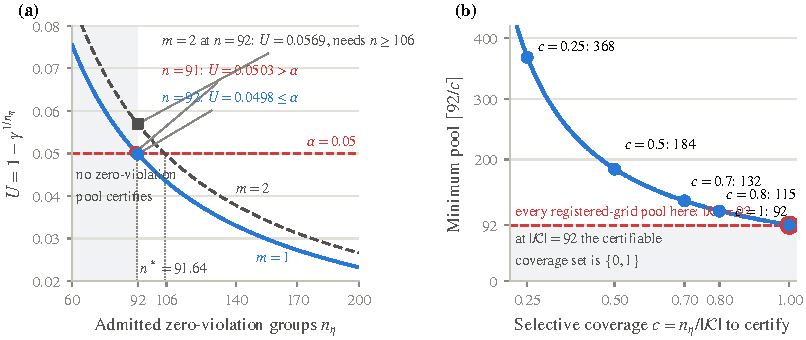
\includegraphics[width=\linewidth]{figures/gate_floor.pdf}
  \caption{Why a 92-group pool certifies only full coverage. (a): the
  zero-violation bound $U(n)=1-(\delta/|\Lambda|)^{1/n}$ at $\delta=0.1$,
  $|\Lambda|=11$ crosses $\alpha=0.05$ between $n=91$ (0.0503) and $n=92$
  (0.0498). (b): the smallest pool $\lceil 92/c\rceil$ that can certify
  selective coverage $c$; every registered-grid calibration pool in this paper
  is 92 (the post-cutoff certificate uses 132 groups under a single rule), so the
  certifiable coverages are 0 and 1 whatever $q$ ranks.}
  \label{fig:gate-floor}
\end{figure}

\paragraph{The nonconformity score $q$.}
$q$ is an $\ell_2$-regularized logistic model over entry-observable features
only --- missing-field indicators, empirical-hull margin, temporal drift, and
provenance ambiguity --- standardized on the development split's own moments so
no calibration statistic enters the fit. Its positive class is an
\emph{unproductive} development group: one the artifact does not carry cleanly
to a verified result, which on $\mathcal{D}$ means a guard rejection, a verifier
abstention, or a manifest mismatch. Wrong executions are not available as
training signal at this point in \cref{alg:compile}, because
\textsc{ReplayAndChallenge} at line~12 retires any candidate that produces one
on $\mathcal{D}$; every candidate reaching \textsc{FitScore} at line~13
therefore has zero contract violations on the development split by construction.
This is a design consequence rather than an oversight --- the cascade is ordered
so that deterministic checks reject before the statistical stage runs --- but it
does mean $q$ is fitted on abstention-shaped supervision and asked at
calibration to rank a different event, which is one plausible reason it
discriminates weakly (\cref{sec:discussion}).

\paragraph{What cohort size permits the gate to certify.}
The zero-violation floor $n_\eta\ge 92$ constrains coverage, not just admission.
Certifying selective coverage $c=n_\eta/|\mathcal{K}|$ requires
$|\mathcal{K}|\ge\lceil 92/c\rceil$: 92 groups for $c=1$, 115 for $c=0.8$, 132
for $c=0.7$, 184 for $c=0.5$. Every registered-grid cohort in this paper fixes
$|\mathcal{K}|=92$ (the post-cutoff certificate's 132 groups use a single rule), which is the smallest pool at which \cref{eq:cp} is
satisfiable at all. At that size the admissible coverage set is exactly
$\{0,1\}$: abstaining on one group leaves $n_\eta=91$ and
$U_\eta=1-(0.1/11)^{1/91}=0.0503>\alpha$. The step-like gate profiles reported
in \cref{tab:gate-profile} and \cref{app:prospective} are therefore consistent
with two different worlds --- a score that cannot rank, and a cohort too small
to certify a ranking --- and these experiments do not separate them. Two
intermediate coverages were \emph{observed} and neither is certifiable:
\code{huggingface/datasets} accepts 10/92 groups at $\eta\le0.08$ in the
gate-frontier study ($U=0.375$), and \code{pandas-dev/pandas} accepts 90/92 at
$0.08\le\eta\le0.20$ in the balanced rerun ($U=0.0509$). A frontier study must
first buy calibration groups (\cref{fig:gate-floor}). The implementation also supports a
minimum-distinct-days requirement, which the single-snapshot live study does not
exercise (\code{min\_days}\,=\,1). Two terms of \cref{eq:score} are coarser in
the implementation than the notation suggests: $\rho_{\mathrm{eff}}$ is
approximated by the fraction of tool names containing a namespace separator
rather than read from the effect catalog, and $|F|$ is substituted by the
argument-slot count of the first observed window because ranking precedes
synthesis. Both affect candidate ranking and thus which candidate is tested, but neither
enters the risk bound. The effect catalog is checked during qualification
and in the runtime facade.

The two executable-gold external substrates are provider-free after their pinned
sources are prepared. Their exact compiler entry points are:
\begin{verbatim}
B=paper/scripts/bfcl_compiler_benchmark.py
python "$B" --source-root "$BENCHMARK_SOURCE_ROOT"
A=paper/scripts/appworld_compiler_benchmark.py
python "$A" --source-root "$BENCHMARK_SOURCE_ROOT" \
  --appworld-python "$APPWORLD_VENV/bin/python"
D=paper/scripts/appworld_dispatch_preflight.py
python "$D" --source-root "$BENCHMARK_SOURCE_ROOT"
\end{verbatim}
The AppWorld environment uses Python~3.12 with package version
\code{0.1.3.post1} and data version \code{0.1.0}; the signed source manifest and
requirements file pin the remaining acquisition inputs. The BFCL source is pinned
to revision \code{6ea57973c7a6}. These commands regenerate only aggregate,
non-sensitive evidence; no model or provider call is made.

\section{Paired Statistics for the Primary Families}
\label{app:stats}

\begin{table}[t]
  \centering
  \caption{Absolute per-record resources behind the percentages of
  \cref{tab:primary}: mean / median over the 30 held-out records of each family
  and over all 90. Estimated dollars are list-price estimates
  (\cref{app:config}); the entire 90-record compiled evaluation cost an
  estimated \$0.028 against \$0.068 for the baseline. Cells are mean / median.}
  \label{tab:absolute-resources}
  \scriptsize
  \setlength{\tabcolsep}{3pt}
  % generated by paper/scripts/iclr_revision_statistics.py absolute; do not edit
\begin{tabular}{@{}llrrrrr@{}}
\toprule
Family & Arm & Requests & Interfaces & Tokens & Latency (ms) & Cost (USD$\times10^{-4}$) \\
\midrule
Issue-type routing & Baseline & 4.00 & 3.00 & 4,259.4 / 4,320 & 6,160 / 5,402 & 8.72 / 8.74 \\
 & Compiled & 2.00 & 3.00 & 2,576.5 / 2,602 & 2,973 / 2,881 & 5.93 / 5.74 \\
 & Manual & 2.00 & 1.00 & 1,780.8 / 1,734 & 3,251 / 2,856 & 5.45 / 5.49 \\
\addlinespace[2pt]
PR-outcome audit & Baseline & 4.00 & 3.00 & 2,718.2 / 2,676 & 5,329 / 4,839 & 6.79 / 6.66 \\
 & Compiled & 1.00 & 1.00 & 521.5 / 462 & 1,440 / 1,297 & 1.68 / 1.51 \\
 & Manual & 1.00 & 1.00 & 522.2 / 458 & 1,827 / 1,364 & 1.69 / 1.51 \\
\addlinespace[2pt]
Backlog-attention routing & Baseline & 3.97 & 2.97 & 2,844.9 / 2,816 & 6,428 / 5,163 & 7.29 / 7.10 \\
 & Compiled & 1.00 & 1.00 & 529.9 / 468 & 2,000 / 1,557 & 1.82 / 1.62 \\
 & Manual & 1.00 & 1.00 & 535.5 / 479 & 1,695 / 1,501 & 1.88 / 1.70 \\
\addlinespace[2pt]
\midrule
All ($n=90$) & Baseline & 3.99 & 2.99 & 3,274.2 / 2,907 & 5,972 / 5,163 & 7.60 / 7.42 \\
 & Compiled & 1.33 & 1.67 & 1,209.3 / 615 & 2,137 / 1,957 & 3.14 / 2.05 \\
 & Manual & 1.33 & 1.00 & 946.2 / 616 & 2,258 / 1,913 & 3.01 / 2.18 \\
\bottomrule
\end{tabular}

\end{table}

\begin{table}[t]
  \centering
  \caption{Per-record paired differences (compiled minus baseline) for all three
  families, with 10{,}000-sample bootstrap intervals (seed 20260802) and
  two-sided Wilcoxon signed-rank tests over $n=30$ paired held-out records
  (exact where differences are tie-free, tie-corrected normal approximation
  otherwise).
  Latency is reported as the mean and as the median paired difference, each with
  its interval; cost intervals are in USD. Provider-request differences are
  deterministic by construction (every pair removes the same number of turns),
  so no rank test is reported for them: the statistic would measure the
  degeneracy rather than the effect. The backlog baseline's one three-request
  record (5189) is the only exception and appears in \cref{tab:discordance}.}
  \label{tab:paired-statistics}
  \footnotesize
  \setlength{\tabcolsep}{3pt}
  % generated by paper/scripts/iclr_revision_statistics.py paired; do not edit
\begin{tabular}{@{}llrr@{}}
\toprule
Family & Endpoint & Paired difference (95\% CI) & $p$ \\
\midrule
\multirow{4}{*}{Issue-type}
 & Total tokens & $-1,682.9\ [-1,772.5,\,-1,596.7]$ & $1.9\times10^{-9}$ \\
 & Wall latency (mean) & $-3,187$\,ms $[-3,758,\,-2,660]$ & $1.9\times10^{-9}$ \\
 & Wall latency (median) & $-2,716$\,ms $[-3,532,\,-2,309]$ & --- \\
 & Estimated cost & $-\$2.79\times10^{-4}\ [-3.13,\,-2.41]\times10^{-4}$ & $3.7\times10^{-9}$ \\
\addlinespace[1pt]
\multirow{4}{*}{PR-outcome}
 & Total tokens & $-2,196.7\ [-2,211.1,\,-2,182.5]$ & $1.7\times10^{-6}$ \\
 & Wall latency (mean) & $-3,889$\,ms $[-4,499,\,-3,346]$ & $1.9\times10^{-9}$ \\
 & Wall latency (median) & $-3,476$\,ms $[-3,736,\,-3,245]$ & --- \\
 & Estimated cost & $-\$5.11\times10^{-4}\ [-5.22,\,-5.02]\times10^{-4}$ & $1.7\times10^{-6}$ \\
\addlinespace[1pt]
\multirow{4}{*}{Backlog-attention}
 & Total tokens & $-2,315.0\ [-2,366.0,\,-2,224.1]$ & $1.7\times10^{-6}$ \\
 & Wall latency (mean) & $-4,428$\,ms $[-5,400,\,-3,558]$ & $1.9\times10^{-9}$ \\
 & Wall latency (median) & $-3,619$\,ms $[-4,201,\,-3,091]$ & --- \\
 & Estimated cost & $-\$5.47\times10^{-4}\ [-5.66,\,-5.23]\times10^{-4}$ & $1.7\times10^{-6}$ \\
\addlinespace[1pt]
\bottomrule
\end{tabular}

\end{table}

\begin{table}[t]
  \centering
  \caption{Exact-contract discordance per family and pooled. ``Baseline-only''
  counts records only the unchanged agent missed; ``compiled-only'' records
  only the compiled arm missed. The upper bound is the one-sided 95\%
  Clopper--Pearson bound on the compiled-only count (0/90 pooled).}
  \label{tab:discordance}
  \footnotesize
  % generated by paper/scripts/iclr_revision_statistics.py paired; do not edit
\begin{tabular}{@{}lrrrrrr@{}}
\toprule
Family & $n$ & Both pass & Baseline-only & Compiled-only & McNemar $p$ & Upper bound \\
\midrule
Issue-type & 30 & 30 & 0 & 0 & 1.00 & 9.5\% \\
PR-outcome & 30 & 30 & 0 & 0 & 1.00 & 9.5\% \\
Backlog-attention & 30 & 29 & 1 & 0 & 1.00 & 9.5\% \\
\midrule
Pooled & 90 & 89 & 1 & 0 & 1.00 & 3.3\% \\
\bottomrule
\end{tabular}

\end{table}

\begin{table}[t]
  \centering
  \caption{Percentage reductions of \cref{tab:primary} with 95\% bootstrap
  intervals on the ratio of paired sums (10{,}000 record resamples, seed
  20260804). Per-family request reductions are structural (backlog's one
  three-request baseline record aside); the intervals on tokens and cost are
  within five points of the estimate, latency within ten.
  Discovery cost alone breaks even after 411, 183, and 181 compiled episodes per
  family and per snapshot (\code{paper/results/cache\_accounting.json}); the
  issue-type baseline's higher cached-input share is why its cost reduction
  trails its token reduction.}
  \label{tab:reduction-ci}
  \footnotesize
  % generated by paper/scripts/iclr_revision_statistics.py paired; do not edit
\begin{tabular}{@{}lrrrr@{}}
\toprule
Family & Requests & Tokens & Latency & Cost \\
\midrule
Issue-type routing & 50.0 [50.0, 50.0] & 39.5 [38.7, 40.3] & 51.7 [46.7, 56.4] & 32.0 [28.3, 35.3] \\
PR-outcome audit & 75.0 [75.0, 75.0] & 80.8 [79.1, 82.5] & 73.0 [68.2, 77.1] & 75.3 [73.3, 77.2] \\
Backlog-attention routing & 74.8 [74.4, 75.0] & 81.4 [79.5, 82.9] & 68.9 [61.4, 75.3] & 75.1 [73.0, 76.9] \\
\midrule
Pooled ($n=90$) & 66.6 [64.1, 68.9] & 63.1 [58.7, 67.8] & 64.2 [60.4, 67.9] & 58.7 [54.1, 63.3] \\
\bottomrule
\end{tabular}

\end{table}

\paragraph{Latency validity.} \Cref{tab:paired-statistics} gives the paired
differences behind \cref{tab:primary}. Latency is wall-clock provider evidence
and is secondary to requests and tokens. In the PR-outcome and backlog families each
held-out record ran its three arms one at a time on one host, cycling through
all six arm orders (five records per order), with no warm-up, a 120\,s
per-episode timeout, and no retries; the issue-type family used a blocked
six-permutation Latin design with eight-way concurrency within each block. No
server-side state is shared between arms (\code{store=False}); cached-input
tokens are zero on every PR-outcome and backlog record and are priced
separately where they occur (\path{paper/results/cache_accounting.json}).
Recomputing the compiled-versus-baseline wall-latency reduction within each of
the six arm orders gives reductions between 43.2\% and 78.6\% across the eighteen permutation--family cells (every cell positive), and
provider-response latency reproduces the wall-latency reductions to within
0.3 percentage points, showing consistency across order blocks while not excluding service variance.

\begin{table}[ht]
  \centering
  \caption{The hand-written comparator priced on the same resource axes as
  \cref{tab:primary}, as percentage reduction against the same baseline and the
  same held-out records. \emph{Manual} is written with full knowledge of the
  workflow, so this is the pessimistic comparison for the compiler: it ties on
  provider requests, issues fewer tool interfaces, and is marginally cheaper in
  tokens and dollars, while compilation leads only on wall latency (bold). The
  interface gap is concentrated in issue-type routing, where the compiled prefix
  covers two reads but the agent still issues the third. We therefore claim
  automated discovery and guarded admission, not runtime dominance over code
  written by someone who already knows the workflow.}
  \label{tab:manual-resources}
  \footnotesize
  \begin{tabular}{@{}lrrrrr@{}}
\toprule
Condition & Requests & Interfaces & Tokens & Latency & Cost \\
\midrule
\multicolumn{6}{@{}l}{\emph{Issue-type routing}} \\
\quad Compiled & 50.0 &  0.0 & 39.5 & \textbf{51.7} & 32.0 \\
\quad Manual   & 50.0 & 66.7 & 58.2 & 47.2 & 37.5 \\
\addlinespace[2pt]
\multicolumn{6}{@{}l}{\emph{PR-outcome audit}} \\
\quad Compiled & 75.0 & 66.7 & 80.8 & \textbf{73.0} & 75.3 \\
\quad Manual   & 75.0 & 66.7 & 80.8 & 65.7 & 75.2 \\
\addlinespace[2pt]
\multicolumn{6}{@{}l}{\emph{Backlog-attention routing}} \\
\quad Compiled & 74.8 & 66.3 & 81.4 & 68.9 & 75.1 \\
\quad Manual   & 74.8 & 66.3 & 81.2 & \textbf{73.6} & 74.2 \\
\midrule
\multicolumn{6}{@{}l}{\emph{Weighted total} ($n=90$)} \\
\quad Compiled & 66.6 & 44.2 & 63.1 & \textbf{64.2} & 58.7 \\
\quad Manual   & 66.6 & 66.5 & 71.1 & 62.2 & 60.4 \\
\bottomrule
\end{tabular}

\end{table}

\paragraph{An extended issue-type held-out cohort.} A pre-registered
extension (\path{paper/supplementary/issue-type-extended-heldout-protocol.md})
ran the retained issue-type artifact on 120 further unused records of the
pinned snapshot on the calibrated model, balanced 40/40/40 over \code{bug},
\code{enhancement}, and \code{other} (the snapshot holds 16 exclusive
\code{question} issues, 10 already used, so the retained three-way mix could
not be reproduced), with the three retained arms in a balanced Latin order and
the artifact recompiled provider-free under the current tracer pin (identical
id, program, splits, and 92/0 gate). By the decision rule fixed in advance the
compiled-only miss comes first: record 2737, where the compiled arm quoted an
error line with backticks the source does not contain; the baseline missed
record 3040 (a doubled space) and all three arms missed record 3968. Exact
contracts were 118/120 baseline, 118/120 compiled, and 117/120 hand-written
(\cref{tab:extended-heldout}); the artifact dispatched on 119/120 records and
abstained cleanly on record 5102 on the induced verifier's cardinality clause,
running the unchanged agent. The one-sided 95\% bound on compiled-only failures
is 3.9\% on these 120 records and 2.2\% pooled with the 90 primary records
(1/210); the pre-registered targets of zero misses, 120/120 dispatch, and a
pooled bound at or below 1.5\% were all missed and are reported as such. Five
of the 120 records had appeared in the gate-frontier pilot's cohort because the
exclusion scan omitted that directory; none of the missed or abstained records
is among them, and without them the counts are 113/113/112 of 115 with bounds
of 4.1\% and 2.3\%.
Requests fell 50.0\%, tokens 39.5\%, latency 42.5\%, and cost 32.8\% against
the same-model baseline, matching the primary family within a point on
requests, tokens, and cost (latency 42.5\% against 51.7\%). In all, 810
held-out GitHub episodes ran under a compiled artifact on the calibrated model
in six studies: 270 on the excerpt-bearing contracts (the 90 primary, these
120, and the 60 post-cutoff records of \cref{app:limits}), with this cohort's
record 2737 the one compiled-only miss (one-sided bound 1.7\%), and 540 on the
outcome-only cross-repository contract (120 core, 180 balanced, and 240
gate-frontier episodes over 354 distinct records; \cref{app:breadth,app:prospective}),
with none.

\begin{table}[t]
  \centering
  \caption{Extended issue-type held-out cohort on the calibrated model:
  per-record means over 120 unused records with a disclosed class mix
  (40 \code{bug} / 40 \code{enhancement} / 40 \code{other}). The compiled-only
  miss (record 2737) and the pooled bound are the pre-registered primary
  endpoints.}
  \label{tab:extended-heldout}
  \footnotesize
  % generated by paper/scripts/issue_type_extended_heldout.py table; do not edit
\begin{tabular}{@{}lrrrrr@{}}
\toprule
Arm & Exact & Requests & Tokens & Latency (s) & Cost (\textcent) \\
\midrule
Unchanged agent & 118/120 & 4.00 & 4,381 & 6.70 & 0.090 \\
Compiled two-read prefix (\method) & 118/120 & 2.00 & 2,649 & 3.85 & 0.061 \\
Hand-written bundle & 117/120 & 2.00 & 1,813 & 3.68 & 0.055 \\
\midrule
\multicolumn{6}{@{}l}{Compiled-only failures: 1/120 here (one-sided 95\% bound 3.9\%);} \\
\multicolumn{6}{@{}l}{1/210 pooled with the primary cohorts (bound 2.2\%)} \\
\bottomrule
\end{tabular}

\end{table}

\section{Additional Experimental Detail}
\label{app:detail}

\begin{table}[t]
  \centering
  \caption{Primary GitHub benchmark at a glance. Each sample supplies one record
  number from a pinned public snapshot; every listed answer field is checked
  against the source record.}
  \label{tab:benchmark-glance}
  \footnotesize
  \setlength{\tabcolsep}{2.5pt}
  \renewcommand{\arraystretch}{1.12}
  \begin{tabularx}{\linewidth}{@{}p{0.16\linewidth}>{\raggedright\arraybackslash}X>{\raggedright\arraybackslash}X@{}}
    \toprule
    Task & Read-only evidence path & Exact answer contract \\
    \midrule
    Issue type & \code{issue\_number} $\rightarrow$ record, official labels,
    comments & Title, state, label-derived category, verbatim excerpt \\
    PR outcome & \code{pr\_number} $\rightarrow$ PR record, merge status,
    discussion & \code{open}, \code{merged}, or \code{closed\_unmerged}, plus
    title and comment excerpt \\
    Backlog attention & \code{issue\_number} $\rightarrow$ open-issue record,
    assignees, discussion & \code{owned}, \code{discussed\_unowned}, or
    \code{awaiting\_first\_response}, plus title, owner, and excerpt \\
    \bottomrule
  \end{tabularx}
\end{table}

\paragraph{Primary workflow families.}
The three-family result is the main paper's strongest live evidence because it
combines distinct tool vocabularies, exact task graders, balanced held-out
cohorts, and provider-backed execution. The compiler limits the issue-type family to
a shallower two-read prefix; the newer pull-request and backlog families
admit deeper pre-model compaction. This difference explains the lower resource
savings on the first family and is part of the evidence boundary, not noise to
average away.

\paragraph{Cross-repository extension.}
The cross-repository study is narrower than the primary workflow families. Its
task uses two read-only tools and a simpler exact outcome contract, which is
precisely why a fixed template can remain tied or even more efficient than the
learned artifact. We keep the result in the main text because it addresses a
central scope question --- whether guarded specialization survives
beyond one repository --- while being explicit about the reduced task complexity.

\paragraph{The position invariant, empirically.}
\label{app:pilot}
An early pilot dispatched a compiled \emph{suffix} region at the entry boundary,
violating \cref{eq:prefix}. Because the runtime resolves artifacts before the
agent has made the calls the region assumed had already happened, the pilot
reordered and duplicated tool calls. The failure is a semantic mismatch between
compilation-time position and resolution-time position, not a tuning error,
which is why \cref{eq:prefix} is a hard constraint in the deployed compiler
rather than a scoring penalty.

\noindent\begin{minipage}{\linewidth}
\paragraph{Omitted from the main claim.}
The repository retains additional studies that are useful scientifically but
less suitable for the main narrative:
\begin{itemize}[leftmargin=1.2em,itemsep=1pt,topsep=2pt]
  \item a natural-order issue study that exposed a factual continuation miss for
  a more aggressive three-read artifact,
  \item exploratory guarded composite synthesis and a follow-up comparison to a
  fair pre-model manual program,
  \item a bounded GEPA prompt-optimization study in which GEPA retained its
  seed, so the combined arm is a replication rather than evidence of
  interaction, and
  \item a portfolio pilot and controlled demonstration suite for runtime
  boundary coverage, including workloads where removing turns \emph{increases}
  cost through prefix-cache fragmentation.
\end{itemize}
\end{minipage}
These studies remain important to the broader artifact, but they either use a
weaker risk level, address a narrower engineering question, or are explicitly
exploratory.

\section{Evidence Breadth and Boundary Audits}
\label{app:breadth}

The main text covers the registered live GitHub studies, the cross-repository
extension, the BIRD live study, and the NESTFUL and AppWorld substrates. This
appendix makes the retained breadth visible without pooling incomparable cohorts
or promoting screened and exploratory work to deployment evidence.

\subsection{Repository-level outcomes on newer records}
The core \code{pytorch/pytorch} run mines one candidate from 116 accepted
windows and retires at calibration. A provider-free recompilation
(\path{paper/results/iclr_revision/pytorch_core_recompile.json}) recovers
$n_\eta=0$ at every threshold, identifying the empty-sample branch of
\cref{eq:cp}. Discovery contains 84 closed-unmerged, 30 open, and 2 merged
records; the held-out split is balanced at 10 per class. The balanced rerun
admits the same task. These observations are consistent with sensitivity to
cohort composition, but neither the degenerate bound nor the rerun establishes
the cause of the original refusal.

\begin{table}[t]
  \centering
  \caption{Held-out dispatch in the cross-repository studies. ``Dispatched''
  counts records on which the compiled program ran; the remainder abstained on
  the named verifier clause and ran the unchanged agent, which is why the
  request reduction is 44.4\% under the core protocol and 66.7\% under the
  balanced one for the same two-read artifact.}
  \label{tab:multirepo-dispatch}
  \footnotesize
  \setlength{\tabcolsep}{3.5pt}
  % generated by paper/scripts/iclr_revision_statistics.py frontier; do not edit
\begin{tabular}{@{}llrrlr@{}}
\toprule
Protocol & Repository & Held-out & Dispatched & Fallback clause & Req.\ $\downarrow$ \\
\midrule
Core & \code{huggingface/datasets} & 30 & 20/30 & \code{range:pr.state} (10) & 44.4\% \\
Core & \code{pandas-dev/pandas} & 30 & 20/30 & \code{range:pr.state} (10) & 44.4\% \\
Core & \code{psf/requests} & 30 & 20/30 & \code{range:pr.state} (10) & 44.4\% \\
Core & \code{pytorch/pytorch} & --- & \textsc{retire} & --- & --- \\
Core & \code{streamlit/streamlit} & 30 & 20/30 & \code{range:pr.state} (10) & 44.4\% \\
\addlinespace[1pt]
Balanced & \code{pandas-dev/pandas} & 60 & 60/60 & --- & 66.7\% \\
Balanced & \code{psf/requests} & 60 & 60/60 & --- & 66.7\% \\
Balanced & \code{pytorch/pytorch} & 60 & 60/60 & --- & 66.7\% \\
\addlinespace[1pt]
\bottomrule
\end{tabular}

\end{table}

\begin{table}[t]
  \centering
  \caption{Disaggregated cross-repository outcomes behind
  \cref{sec:res-multirepo}.
  The core protocol uses four completed repositories and one compile-time
  retirement; the balanced rerun changes the selected repositories and class
  mix, so it is reported separately rather than pooled with the core protocol.
  Reductions compare the compiled condition with the paired unchanged baseline.}
  \label{tab:multirepo-disaggregated}
  \footnotesize
  \setlength{\tabcolsep}{3.5pt}
  \begin{tabular}{@{}llrrrr@{}}
\toprule
Protocol & Repository & Held-out & Exact & Req. $\downarrow$ & Tokens $\downarrow$ \\
\midrule
Core & huggingface/datasets & 30 & 30/30 & 44.4\% & 52.2\% \\
Core & pandas-dev/pandas   & 30 & 30/30 & 44.4\% & 52.5\% \\
Core & psf/requests        & 30 & 30/30 & 44.4\% & 52.3\% \\
Core & streamlit/streamlit & 30 & 30/30 & 44.4\% & 52.7\% \\
Core & pytorch/pytorch     & --- & \textsc{retire} & --- & --- \\
\addlinespace[1pt]
Balanced & pandas-dev/pandas & 60 & 60/60 & 66.7\% & 78.6\% \\
Balanced & psf/requests      & 60 & 60/60 & 66.7\% & 78.7\% \\
Balanced & pytorch/pytorch   & 60 & 60/60 & 66.7\% & 78.0\% \\
\bottomrule
\end{tabular}

\end{table}

The core result succeeds on four repositories (120/120 held-out pairs) and
retains the fifth as a compile-time retirement after 116 exact discovery traces.
The balanced rerun has a distinct three-repository cohort and reaches 180/180
held-out pairs. These rows show breadth across repositories drawn from shared
pools --- the balanced rerun shares 13, 25, and 8 of the 30-record core
held-out sets --- not independent evidence for an average effect: all runs
share the same provider family and the same narrow two-read outcome task.

\subsection{Continuation audit}

The earlier natural-order three-read study is excluded from the registered
$\alpha=0.05$ headline because it used $\alpha=0.10$ and exposed a downstream
continuation error. Its retained counterfactual replay nevertheless tests a
boundary the exact tool contract cannot see: 17/18 candidate continuations pass
unchanged, while issue 6602 has a comment-evidence mismatch. Checked rendering
repairs that one case, yielding 18/18 final contracts. This audit makes no
provider calls and does not estimate live agent quality; it establishes only
that the continuation check caught a concrete failure the compacted tool trace
alone would miss.

\subsection{External evidence map}
\label{app:external}

\begin{table}[t]
  \centering
  \caption{All four trace benchmarks used as compiler substrates. NESTFUL and
  AppWorld are discussed in \cref{sec:res-refusal}; API-Bank and executed BFCL
  v4 gold plans retire on support exactly like NESTFUL. Columns as in
  \cref{tab:funnel}.}
  \label{tab:funnel-all}
  \footnotesize
  \setlength{\tabcolsep}{4pt}
  \begin{tabular}{@{}lrrrrrcrc@{}}
\toprule
Substrate & Traces & Slots (1) & Windows (2) & At floor (2) & Synth.\ (4) & Replay p/a/\textbf{w} (5) & $n_{\max}$ (6) & Adm. \\
\midrule
NESTFUL   & 1{,}415 & 96.3\% & 1{,}207 & 32 & 12 & 24 / 12 / \textbf{0} & 26 & \textbf{0} \\
API-Bank  &     212 & 63.5\% &      37 &  8 &  2 &  0 /  2 / \textbf{0} &  8 & \textbf{0} \\
BFCL v4   &     200 & 68.0\% &      86 &  9 &  4 &  3 /  3 / \textbf{0} & 15 & \textbf{0} \\
AppWorld  &     136 & 63.2\% &     136 & 33 &  1 & 34 /  0 / \textbf{0} & \textbf{136} & \textbf{1} \\
\bottomrule
\end{tabular}

\end{table}


\Cref{tab:external-evidence-map} records every named external benchmark in the
retained evidence register and its admissible interpretation.

\paragraph{Obtaining observed results from BFCL.}
BFCL's reference plans carry no tool results, which is why the plan-format row
and the compiler row are listed separately. Its multi-turn categories, however,
ship an executable stateful backend: each task publishes an
\code{initial\_config} snapshot and the classes it involves, so executing the
\emph{official gold plan} through the upstream helper yields observed results,
an entry snapshot, and an in-process replay oracle, with no model in the loop.
Five preconditions fail the run closed rather than publishing: an undeclared
method, any upstream execution error, a read-like declaration observed mutating
state, a compilable declaration observed advancing the scenario RNG, and any
inexact re-execution. All held: 200 tasks and 1{,}142 calls executed cleanly and
a second independent pass reproduced every result byte for byte, executing
turn-at-a-time where the first pass executed call-at-a-time.

\paragraph{Why the catalog is signed rather than inferred.}
The same run audits the declarations empirically by snapshotting every involved
instance around every call. It observed 1{,}060 state-mutating calls over 44 of
the 81 methods and 94 calls that advanced the seeded scenario RNG, with zero
cases of a read-like declaration mutating state or a compilable declaration
advancing the RNG. One case is worth naming: a method whose name and docstring
present it as a cost getter mutated its instance's internal lookup on all 36 of
its calls and is therefore declared a write. A name- or docstring-derived effect
label would have admitted a write into a compiled region. Two further methods
are read-like but carry no capabilities, because one derives an age from the
host date and the other draws from --- and advances --- the seeded RNG; they are
barriers by declaration and account for 35 suppressed spans. Write barriers
suppress 2{,}802 spans in total, against 45 for entry-schema admissibility, 31
for slot ambiguity, and 5 for partial runs.

\paragraph{Obtaining observed results from AppWorld, and why it is the reachable case.}
AppWorld's shipped \code{api\_calls.json} records method, url, and request data
but no responses, so it fails closed for the same reason BFCL's plans do.
Executing the official \code{compiled\_solution\_code} against the pinned
\code{0.1.3.post1} backend supplies the results; each task's own
\code{specs.json} supplies the entry snapshot; a second execution supplies the
replay oracle. Calls are captured at the single dispatch point every
\code{apis.<app>.<api>(...)} call passes through, so the recorded identity is a
semantic app/API pair with typed keyword arguments and a decoded JSON result. Of
the 147 public train+dev gold solutions, 136 execute cleanly; 11 dev solutions
raise against the shipped data version and are reported as upstream
compatibility outcomes rather than dropped. The second pass reproduced
7{,}070/7{,}070 results byte for byte, minted access tokens included, because
AppWorld freezes each task's clock.

The empirical audit attributes every
\code{INSERT}/\code{UPDATE}/\code{DELETE}/\allowbreak\code{CREATE}/\code{DROP} statement to the enclosing call. It observed 1{,}320
mutating calls, zero read-like declarations mutating, and --- unlike BFCL --- zero
APIs that mutate on some calls but not others. Every \code{GET} was clean on
every call and every \code{DELETE} and \code{PATCH} mutated on every call, so
the effect boundary is crisp; the five \code{*.login} endpoints are the only
non-\code{GET} APIs that never mutate, which is why they are the single
contestable declaration and why the run is pre-registered in two arms. Groups
are tasks, not scenarios: AppWorld's three variants of a scenario share a
supervisor and a database, so the bound is conditional on task-level
independence, which this corpus does not establish --- the same conditional the
live studies carry, neither weakened nor repaired here; at scenario or
supervisor level (46 and 79 units) the zero-violation bound is 0.097 and
0.058, both above $\alpha$. Arm A calibrated one candidate and is
compiler-wide; arm B calibrated six (four retired, one dominated, one emitted),
so its certificate is per-candidate, with a corrected bound of 0.068. The calibration share is
fixed at exactly the 92 groups the bound needs, since a larger set would make
the bound easier and a smaller one would make it unreachable. Two held-out
replay figures appear for AppWorld and they count different partitions, which
\cref{tab:funnel} flags but does not have room to explain. The 34/0/0 in that
table is the test side of the \emph{family} partition used to challenge a mined
candidate --- 102 train and 34 test groups, the same accounting every substrate
row reports. The separately reported 11/11 admission-test passes are from the sealed test split
of the 11/92/11 dev/calibration/test partition \cref{alg:calibrate} consumes for
admission. Both are genuinely held out; they are held out from different fits,
and neither is a subset of the other's training side.

\begin{table}[t]
  \centering
  \caption{Structural dispatch eligibility of the admitted AppWorld artifact on
  the 28 released official baseline runs. Eligibility is the admitted program's
  exact call sequence at normalized position~0; it is an upper bound on $\varphi$,
  because the manifest check and the calibrated gate are not evaluated and the
  released logs retain API calls rather than model boundaries. Trajectories repeat
  tasks across runs and are descriptive rather than independent samples. A miss
  abstains to the unchanged agent.}
  \label{tab:appworld-dispatch}
  \footnotesize
  \setlength{\tabcolsep}{5pt}
  \begin{tabular}{@{}lrrrr@{}}
\toprule
Released baseline architecture & Runs & Trajectories & Eligible at pos.~0 & Rate \\
\midrule
Full code + reflection                & 8 & 2{,}340 & 2{,}339 & 1.000 \\
Iterative parallel function calling   & 4 & 1{,}170 &    762 & 0.651 \\
Plan and execute                      & 8 & 2{,}340 &      1 & 0.000 \\
ReAct                                 & 8 & 2{,}340 &      0 & 0.000 \\
\midrule
Pooled                                & 28 & 8{,}190 & 3{,}102 & 0.379 \\
\bottomrule
\end{tabular}

\end{table}

\paragraph{Admissible is not dispatchable.}
\Cref{tab:appworld-dispatch} separates the two. The admitted region is eligible
on essentially every full-code trajectory and essentially no ReAct or
plan-and-execute trajectory, because those architectures open by reading API
documentation---3{,}752 of the 8{,}190 released trajectories begin with an
API-description call --- so the compiled prefix is no longer at position~0 and
\eqref{eq:prefix} refuses. A further 61 trajectories contain the program
somewhere other than position~0, which the same invariant refuses. Full-code
agents are eligible on $2{,}339/2{,}340$ trajectories and iterative parallel
function-calling agents on $762/1{,}170$. Two secondary observations: the rate
is flat across task difficulty ($0.377$ on \code{test\_normal} against $0.380$
on \code{test\_challenge}), consistent with the strong association with agent architecture, without
excluding workload effects; and the maximal compilable depth is 2 on the eligible
families, so the admitted two-step program sits at the ceiling the effect
catalog permits rather than short of it. On the ineligible families the measured
depth is a floor, not an estimate, because the API-documentation call is
undeclared in the signed catalog and unknown effects are not reads.

\begin{table}[t]
  \centering
  \caption{Disposition of every retained external benchmark family. Only the
  four compiler-measurement rows and the BIRD live study support compiler claims; the remaining rows
  document why broader benchmark names are not silently converted into GAC
  results. BFCL appears twice because its reference plans and its executed gold
  plans are different evidence.}
  \label{tab:external-evidence-map}
  \footnotesize
  \setlength{\tabcolsep}{3pt}
  \renewcommand{\arraystretch}{1.05}
  \begin{tabularx}{\linewidth}{@{}l >{\raggedright\arraybackslash}p{0.28\linewidth} >{\raggedright\arraybackslash}X@{}}
\toprule
Benchmark & Evidence tier & Retained result / claim boundary \\
\midrule
NESTFUL & Compiler measurement & 1{,}415 traces; 24 / 12 / 0 replay; all families retire. \\
API-Bank & Compiler measurement & 212 traces; 0 / 2 / 0 replay; all candidates retire. \\
BFCL v4 (plans) & Gold-plan checker & 200/200 valid plans; plan format only. \\
BFCL v4 (executed) & Compiler measurement & 200 traces, 1{,}142/1{,}142 exact re-execution; 3 / 3 / 0 replay; all families retire. \\
AppWorld (executed) & Compiler measurement & 136/147 traces, 7{,}070/7{,}070 exact re-execution; $n_{\max}=136\ge92$; one artifact admitted at $U=0.0498$; under arm B two candidates retire at the margin ($U=0.051$) and two far from it ($U=1$). \\
BIRD (dev and train) & Live-provider compiler study & 31 databases, two agent designs, three models: the standard design retires everywhere; the schema-first opening is admitted on 26 of 31 databases (\code{gpt-5.6-luna}) and 5 of 5 (\code{gpt-6-luna}); no detected accuracy loss on 924 held-out questions (\cref{app:bird}). \\
ToolSandbox & Live-provider subset & One simulated scenario; compiler not run. \\
$\tau^2/\tau^3$ & Live-provider subset & 0/4 pass; compiler not run. \\
ToolBench & Adapter smoke & Ten fixtures; full data/backend unavailable. \\
AgentBench & Adapter/preflight & Services and Freebase data gated. \\
GAIA & Access preflight & Authorization denied; no metric. \\
SWE-bench Verified & Task adapter & Official run host-gated. \\
BrowseComp & Live-web subset & 1/3 correct, 28 searches; bypassed by the compiler. \\
\bottomrule
\end{tabularx}

\end{table}

\subsection{A live agent on a public benchmark: BIRD}
\label{app:bird}

\paragraph{Design.} The study was registered before any provider call
(\path{paper/supplementary/bird-sql-agent-protocol.md}). A tool-using SQL agent
on \code{gpt-5.6-luna}, with the paper's pinned settings, answers BIRD dev
questions~\citep{li2023bird} (release \code{dev\_20240627}, question plus
evidence) over read-only SQLite files with three tools: \code{list\_tables},
\code{get\_schema(table\_names)} with three sample rows, and \code{run\_query}.
The contract is BIRD execution accuracy: the final query's result set equals
the gold query's. Every dev database with at least 146 questions (16 train, 8
dev, 92 calibration, 30 held out) is a family, which selects five. Two agent
designs were registered: \emph{standard}, adapted from LangChain's SQL-agent
prompt \citep{langchain2026sql} (``query the schema of the most relevant tables''), and
\emph{schema-first}, whose workflow step reads every table before writing a
query, the analogue of the paper's prescribed design. QUALIFY does not filter
on answer correctness, the compiler runs with the registered settings, and a
strict audit vetoes any admission whose calibration groups show the agent
passing different opening arguments than the program derives.

\begin{table}[t]
  \centering
  \caption{BIRD: compile-or-retire per database and design, and the schema-first
  held-out evaluation (30 sealed questions per database). ``Repeat'' is a
  second independent run of the unchanged agent. Reductions compare the
  compiled agent with that warm-cache repeat run (the condition order was not
  rotated as registered; see text). Standard-design retirements are at
  synthesis (\code{ungroundable\_slot}) or on calibration support.}
  \label{tab:bird}
  \footnotesize
  \setlength{\tabcolsep}{3pt}
  \resizebox{\linewidth}{!}{% generated by paper/scripts/bird_sql_agent_study.py --phase summarize; do not edit
\begin{tabular}{@{}lrlccccrrr@{}}
\toprule
& & Standard & \multicolumn{4}{c}{Schema-first: correct of 30} & \multicolumn{3}{c}{Compiled vs.\ warm repeat} \\
\cmidrule(lr){3-3}\cmidrule(lr){4-7}\cmidrule(l){8-10}
Database & Tables & GAC & Base & Repeat & Compiled & Manual & Requests & Tokens & Cost \\
\midrule
\code{card\_games} & 6 & retire: support 34/92 & 18 & 16 & \textbf{19} & 18 & 44.1\% & 7.8\% & $-$2.6\% \\
\code{codebase\_community} & 8 & retire: synthesis & 22 & 23 & \textbf{22} & 21 & 48.8\% & 15.2\% & 6.3\% \\
\code{formula\_1} & 13 & retire: synthesis & 18 & 19 & \textbf{20} & 19 & 43.7\% & 4.2\% & 1.8\% \\
\code{student\_club} & 8 & retire: synthesis & 26 & 25 & \textbf{24} & 24 & 49.6\% & 19.0\% & 18.7\% \\
\code{thrombosis\_prediction} & 3 & retire: synthesis & 10 & 11 & \textbf{12} & 12 & 39.0\% & 6.0\% & 12.1\% \\
\midrule
Pooled & & 5 retire & 94 & 94 & \textbf{97} & 94 & 44.9\% & 9.8\% & 6.3\% \\
\bottomrule
\end{tabular}
}
\end{table}

\paragraph{Admission.} The standard agent passed 7 to 39 distinct table lists
per database and every table in no discovery run on four of them, so
\code{get\_schema.table\_names} has no consistent expression and four families
retire at synthesis (\cref{tab:bird}). On \code{card\_games} the candidate
``read only \code{cards}'' (the agent's most common choice, 61 of 132 runs)
matched 34 calibration groups and retired on support. In 7 of those groups the
agent had read a different table; the compiler labeled them unproductive, which
stays in the count, rather than violations. That is the leniency the strict
audit was registered to catch, and with more support the compiler alone could
have admitted a wrong-shaped program. The schema-first agent passed the full
listing in every discovery run, and every family admitted
\code{list\_tables} $\to$ \code{get\_schema}(all tables) with one candidate at
calibration (compiler-wide), 92 groups, zero violations, and a clean audit. The
table list is bound as an invariant literal, not as an expression over the
listing as the protocol predicted, because the implemented rule tries literals
first.

\paragraph{Held-out evaluation.} The compiled program dispatched on 150 of 150
sealed questions. Execution accuracy was 97/150 compiled, 94/150 for the
unchanged agent, 94/150 for its repeat, and 94/150 for a hand-written schema
prefetch; compiled against the unchanged agent there are 5 compiled-only and 2
baseline-only correct answers (McNemar $p=0.45$; difference $+2.0$ points,
95\% interval $[-1.3,+5.3]$), which meets the registered criterion for no
detected accuracy loss. The interval also permits a loss; neither equivalence
nor noninferiority was established. The registered rotation
of condition order was not implemented: the four conditions ran in a fixed
order, so the first baseline met a colder provider prompt cache (cached-input
share 0.504 against 0.56--0.59) and its repeat was 11.9\% cheaper with the same
tokens. Against the warm repeat, the compiled agent made 44.9\% fewer model
requests $[42.1,47.4]$, used 9.8\% fewer tokens $[4.7,14.3]$, ran 29.4\% faster
$[23.6,35.1]$, and cost 6.3\% less $[1.5,10.6]$; against the first run the cost
reduction is 17.5\%, and pricing every input token at the uncached rate gives
11--12\% either way. The hand-written prefetch reaches 46.3\%, 12.4\%, 31.5\%,
and 7.9\%, so the discovered program matches the manual ceiling. Savings in
tokens and cost are modest because the two removed calls carry the shortest
contexts. Total spend was \$2.69.

\paragraph{Extensions: order, models, providers, and scale.} Four extensions
were registered before any of their provider calls
(\path{paper/supplementary/bird-sql-agent-extensions-protocol.md};
\cref{tab:bird-extensions}). A rerun with the condition order rotated as
originally registered reproduces the result on the same 150 questions (100
against 94 correct; McNemar $p=0.07$, no superiority claimed) with 46.0\% fewer
requests and 16.2\% lower cost against the first baseline. On a second model
family, \code{gpt-6-luna}, the standard design retires on all five databases and
the schema-first opening is admitted on all five, with 49.9\% fewer requests and
93 against 91 correct on 149 complete-case questions (150 were scheduled). On the BIRD training split (26 databases
with at least 146 questions, after a pre-execution rule excluded one whose gold
SQL references tables missing from the shipped database), the standard design
retires on all 26 and the schema-first opening is admitted on 21; the five
refusals are databases (11 to 65 tables) where the agent occasionally dropped or
reordered a table, four on calibration support (90 or 91 of 92
groups) and one at synthesis. On the 625 four-arm-complete questions across the 21 admitted
databases the compiled agent dispatched every time and answered 400 correctly
against 401 ($p=1.0$), with 45.9\% fewer requests, 12.6\% fewer tokens, 29.3\%
lower latency, and 18.1\% lower cost. Pricing every input token at the uncached
rate, which removes provider-cache effects, gives cost reductions of 11--18\% in
every run. On a second provider, Anthropic \code{claude-sonnet-5}, the agent
followed neither opening as a fixed step: under the schema-first prompt it
listed the tables first in 429 of 655 runs and passed every table in 26, and
\method retired all ten (design, database) pairs. \method compiles what an agent
does, not what its prompt asks for. Extension spend was \$43.93.

\begin{table}[t]
  \centering
  \caption{BIRD runs. ``Std.'' and ``S.-first'' count databases admitted per
  design (the rotated rerun reuses the primary artifacts). Correct is on the
  held-out questions completed by all four conditions; bold marks the compiled arm,
not a significant improvement. Reductions compare the compiled
  agent with the unchanged agent; $^\dagger$every primary-row reduction is against
  the warm repeat run because that run's order was not rotated. Cost$^\ast$ prices every input token
  at the uncached rate.}
  \label{tab:bird-extensions}
  \footnotesize
  \resizebox{\linewidth}{!}{% generated by paper/scripts/bird_sql_agent_study.py --phase extensions-table; do not edit
\begin{tabular}{@{}llcccccrrrrr@{}}
\toprule
Run & Model & DBs & Std. & S.-first & $n$ & Correct (base / GAC) & Requests & Tokens & Latency & Cost & Cost$^\ast$ \\
\midrule
Primary (fixed order) & \code{gpt-5.6-luna} & 5 & 0 & 5 & 150 & 94 / \textbf{97} & 44.9\% & 9.8\% & 29.4\% & 6.3\%$^\dagger$ & 11.2\% \\
E1 rotated rerun & \code{gpt-5.6-luna} & 5 & --- & --- & 150 & 94 / \textbf{100} & 46.0\% & 12.3\% & 33.9\% & 16.2\% & 13.9\% \\
E2 second model & \code{gpt-6-luna} & 5 & 0 & 5 & 149 & 91 / \textbf{93} & 49.9\% & 16.8\% & 38.4\% & 6.1\% & 17.5\% \\
E3 second provider & \code{claude-sonnet-5} & 5 & 0 & 0 & --- & --- & --- & --- & --- & --- & --- \\
E4 train split & \code{gpt-5.6-luna} & 26 & 0 & 21 & 625 & 401 / \textbf{400} & 45.9\% & 12.6\% & 29.3\% & 18.1\% & 14.0\% \\
\bottomrule
\end{tabular}
}
\end{table}

\paragraph{Attrition and all-scheduled denominators.}
The historical summaries above retain only questions completed by all four
arms. This excludes one second-model question because the repeat baseline
 timed out, and five training-split questions: four manual-arm timeouts and
one compiled-arm turn-limit failure. A retrospective audit of the sealed run
records counts every scheduled question, treating each missing run as incorrect
only in its own arm (\cref{tab:bird-denominators}). Training-split accuracy is
402/630 compiled versus 403/630 unchanged, with 17 compiled-only and 18
baseline-only correct ($p=1$); second-model accuracy is 93/150 versus 91/150
($p=0.73$). Neither result establishes noninferiority. Resource comparisons
require completed runs: using all baseline/compiled pairs gives request/cost
reductions of 45.8/18.0\% on 629 training pairs and 49.6/5.8\% on 150
second-model pairs. These estimates omit resources consumed by failed runs;
aggregate billed cost and time-to-success are not established by them.
The script \path{paper/scripts/audit_bird_denominators.py} regenerates these
counts without provider calls. The pinned BIRD release is
\code{dev\_20240627}; these selected-family results are not a leaderboard score
on the newer cleaned development set.

\begin{table}[t]
  \centering
  \caption{Retrospective BIRD quality over all scheduled questions. Missing
  runs count as incorrect in their own arm; ``Complete'' is the historical
  four-arm intersection. Rotated repeats the primary questions.}
  \label{tab:bird-denominators}
  \footnotesize
  % generated by paper/scripts/audit_bird_denominators.py; do not edit
\begin{tabular}{@{}lrrrrrr@{}}
\toprule
Run & Scheduled & Complete & Base & Repeat & GAC & Manual \\
\midrule
Primary & 150 & 150 & 94 & 94 & 97 & 94 \\
Rotated & 150 & 150 & 94 & 93 & 100 & 96 \\
Second model & 150 & 149 & 91 & 95 & 93 & 90 \\
Train split & 630 & 625 & 403 & 412 & 402 & 404 \\
\bottomrule
\end{tabular}

\end{table}

\paragraph{How much quality loss remains compatible with the data?}
The all-scheduled audit supports a retrospective uncertainty analysis
(\cref{tab:bird-quality-sensitivity}), without selecting a noninferiority margin
after seeing the results. Let $p_+$ denote the probability of a compiled-only
correct answer and $p_-$ a baseline-only correct answer. The paired accuracy
difference is $\Delta=p_+-p_-$. Construct a two-sided 97.5\% Clopper--Pearson
interval for each probability \citep{clopper1934binomial}; if their endpoints are
$[L_+,U_+]$ and $[L_-,U_-]$, then $[L_+-U_-,U_+-L_-]$ covers $\Delta$ with
at least 95\% probability under i.i.d.\ question pairs, by a union bound.
Dependence between the gain and loss indicators within a pair is allowed.
These conservative, pointwise intervals are wider than the primary study's
paired bootstrap interval; neither construction proves the sampling assumption.
They are not simultaneous across the four rows, and overlapping primary,
rotated, and second-model questions are not pooled as independent evidence.

\begin{table}[t]
  \centering
  \caption{Retrospective BIRD quality sensitivity on all scheduled questions.
  All differences are compiled minus unchanged, in percentage points.
  Intervals assume i.i.d.\ question pairs. ``Delete-one'' omits each entire
  database in turn; it is a descriptive range, not a confidence interval.
  The last column counts databases with positive, zero, or negative differences.}
  \label{tab:bird-quality-sensitivity}
  \footnotesize
  \resizebox{\linewidth}{!}{% generated by paper/scripts/bird_quality_sensitivity.py; do not edit
\begin{tabular}{@{}lrrrr@{}}
\toprule
Cohort & $\Delta$ (pp) & Conservative 95\% interval & Delete-one range & DBs $+/0/-$ \\
\midrule
Primary & $+2.00$ & $[-4.40, +8.18]$ & $[+0.83, +4.17]$ & 3/1/1 \\
Rotated & $+4.00$ & $[-2.53, +10.11]$ & $[+1.67, +5.83]$ & 3/1/1 \\
Second model & $+1.33$ & $[-5.44, +7.97]$ & $[-0.83, +3.33]$ & 3/0/2 \\
Train split & $-0.16$ & $[-3.27, +2.96]$ & $[-0.50, +0.33]$ & 5/10/6 \\
\bottomrule
\end{tabular}
}
\end{table}

The training interval allows a loss of 3.27 points or a gain of 2.96 points.
Deleting one database keeps its observed difference between $-0.50$ and
$+0.33$ points; 5 databases favor the compiled agent, 10 tie, and 6 favor the
unchanged agent. The second-model difference changes sign under a database
deletion. This tests concentration of the observed result, without treating
the selected databases as a random sample or establishing generalization to
new databases. The retained script \path{paper/scripts/bird_quality_sensitivity.py}
regenerates the intervals, database deletions, and source hashes.

\paragraph{Sensitivity to missing execution cost.}
The same training records retain \$0.891759 of estimated cost for 630 completed
baseline runs and \$0.728806 for 629 completed compiled runs. Let $u\ge0$ be
the unrecorded cost of the single failed compiled execution, priced with the
same frozen rate card. Net evaluation savings are then
\$0.162952 minus $u$, so they are positive only if $u<\$0.162952$.
This is a break-even condition, not evidence that the unknown cost satisfies
it. It includes the failure's quality penalty above but cannot recover its
missing usage; discovery, recompilation, and maintenance remain excluded.

\subsection{The registered gate is a support threshold}

This audit strengthens the evidentiary record precisely by preserving the
negative result: the registered gate behaves as, and at $|\mathcal{K}|=92$ can
only behave as, a support threshold rather than a demonstrated risk--coverage
frontier (\cref{tab:gate-profile}); the question of $q$'s ranking quality is
open, not answered negatively. The exploratory partial frontiers therefore
remain diagnostic rather than evidence for the main claim.

\begin{table}[t]
  \centering
  \caption{Gate-behavior inventory from the retained threshold analysis. A
  partial frontier would show graded coverage as the threshold changes; none
  appears among the seven artifacts in the retained threshold analysis.}
  \label{tab:gate-profile}
  \footnotesize
  \setlength{\tabcolsep}{4pt}
  \begin{tabularx}{\linewidth}{@{}lrr>{\raggedright\arraybackslash}X@{}}
\toprule
Evidence set & Artifacts & Partial frontiers & What it licenses \\
\midrule
Registered GitHub $\alpha=0.05$ (threshold analysis) & 7 & 0 & Exact per-candidate certificates; all are step-like. \\
Exploratory or looser-$\alpha$ & 3 & 2 & Diagnostic evidence only; not the registered claim. \\
NESTFUL refusal & 12 synthesized & 0 & $n_{\max}=26<92$; no admission. \\
API-Bank refusal & 2 synthesized & 0 & $n_{\max}=8<92$; no admission. \\
BFCL v4 refusal & 4 synthesized & 0 & $n_{\max}=15<92$; no admission, pre-registered. \\
AppWorld admission & 1 admitted / 4 retired & 0 & $n_{\max}=136\ge92$; the one reachable external bound. Admitted gate is step-like; two retirements are marginal ($U=0.051$ at 89 and 90 eligible groups), two are not ($U=1$). \\
\bottomrule
\end{tabularx}

\end{table}

\section{Extended Limitations}
\label{app:limits}

Every protocol in this paper is in-repo and author-held; no external registry
was used, and each is dated in its own file.

\paragraph{The certified event is not end-to-end quality.}
\Cref{prop:admission} bounds the replay-contract event of \cref{app:config}.
On these cohorts that event has no empirical support: the argument pattern of
the compiled steps is invariant across all discovery traces per GitHub family,
and the labels replay those calls over recorded results of a pinned snapshot,
which is why no retained pool records a violation, every gate is step-like,
and admission reduces to the 92-group floor (the second-provider backlog
refusal turns on 90 and 91 eligible groups). The misses that do occur on these families are
continuation misses (an excerpt that departs from its source), and they are
outside the certificate: the one-sided 95\% upper bound on compiled-only
discordance in \cref{app:stats} is an empirical quality statement at a
different confidence level, not an admission certificate. An end-to-end
certificate needs a pre-registered endpoint that runs the continuation and
grades the task contract on fresh calibration groups, with the sample floor of
\cref{eq:cp} applied to that event; one was obtained after the main study for a
re-derived PR-outcome artifact on 132 fresh groups (0 misses, bound 0.0173 at
90\% confidence; below), and is reported separately from the primary replay-contract certificates.

\paragraph{Dependence sensitivity.}
The exact binomial bound requires i.i.d. units. One valid cluster-level
formulation uses i.i.d. clusters and the maximum violation within each cluster,
targeting risk for a new cluster rather than a new record. Distinct days or
authors do not establish that assumption; \cref{tab:effective-units} is a
hypothetical sensitivity calculation. Temporal spacing alone does not ensure
independence, and block bootstrap or dependence-aware conformal methods require
their own assumptions and guarantees; they do not inherit \cref{eq:cp}.
For clean-checkout reproduction, the retained
\path{paper/results/iclr_revision/calibration_cluster_rows.json} records the
calibration row identifiers, dates, and hashed author equality keys derived
from the digest-checked source snapshots.

\begin{table}[t]
  \centering
  \caption{Distinct grouping units in the 92-record calibration cohorts,
  joined to the pinned snapshot: distinct creation days, months, and authors,
  and the zero-violation bound the registered budget would give if each cluster
  were one unit (admits only when the count is at least 92).}
  \label{tab:effective-units}
  \footnotesize
  \setlength{\tabcolsep}{4pt}
  % generated by paper/scripts/iclr_revision_statistics.py clusters; do not edit
\begin{tabular}{@{}lrrrrrr@{}}
\toprule
Cohort & $n$ & Days & Months & Authors & $U$ at days & $U$ at authors \\
\midrule
Issue-type routing & 92 & 90 & 50 & 82 & 0.051 & 0.056 \\
PR-outcome audit & 92 & 86 & 45 & 60 & 0.053 & 0.075 \\
Backlog-attention routing & 92 & 87 & 46 & 73 & 0.053 & 0.062 \\
Core: \code{huggingface/datasets} & 92 & 80 & 37 & 46 & 0.057 & 0.097 \\
Core: \code{pandas-dev/pandas} & 92 & 92 & 66 & 53 & 0.050 & 0.085 \\
Core: \code{psf/requests} & 92 & 90 & 66 & 79 & 0.051 & 0.058 \\
Core: \code{streamlit/streamlit} & 92 & 87 & 33 & 25 & 0.053 & 0.171 \\
\bottomrule
\end{tabular}

\end{table}

\paragraph{A read-only prologue does not recover ReAct dispatch.}
\Cref{sec:res-refusal} shows \cref{eq:prefix} refuses essentially every ReAct
and plan-and-execute trajectory, which open with an API-documentation read. We
built the narrowest relaxation
(\path{paper/supplementary/read-only-prologue-protocol.md}): an artifact may
declare an exact, allowlisted, read-only prologue whose calls must equal the
committed observations in tool, order, and arguments; the prologue's results
become live-ins of the region, its calls are not replayed, and any mismatch,
extra call, order change, manifest mismatch, unknown effect, or slot left
ungrounded by the extended entry contract falls back. The runtime passes the
protocol's acceptance tests, including the archived suffix-dispatch pilot as a
regression test. Measured on the 8{,}190 released trajectories with the
documentation call as the prologue (\cref{tab:appworld-prologue}), it changes little: ReAct eligibility rises from 0 to 2 of 2{,}340 and plan-and-execute
stays at 1. The looser diagnostic --- any documentation-only prefix followed by
the admitted program --- recovers 2 and 3, and the program occurs anywhere in
only 16 and 39 of those trajectories. Position was the proximate reason those
architectures were refused; the larger limitation is that they seldom execute the
admitted region at all. A prologue rule cannot recover those absent executions. The prologue tool
is also undeclared in the signed catalog, and the runtime refuses an undeclared
prologue; the measurement assumes the declaration a reviewer would have to sign.

\begin{table}[t]
  \centering
  \caption{Structural dispatch eligibility before and after admitting an exact
  read-only prologue (the API-documentation call these architectures open
  with), per released AppWorld baseline architecture; never pooled. The
  runtime rule and the measurement rule are the same function.}
  \label{tab:appworld-prologue}
  \scriptsize
  \setlength{\tabcolsep}{3pt}
  \begin{tabular}{@{}lrrrrrr@{}}
\toprule
Released baseline architecture & Runs & Trajectories & Before (pos.~0) & Rate & After (pos.~0 or exact prologue) & Rate \\
\midrule
Full code + reflection                 & 8 & 2{,}340 & 2{,}339 & 1.000 & 2{,}339 & 1.000 \\
Iterative parallel function calling    & 4 & 1{,}170 & 762 & 0.651 & 762 & 0.651 \\
Plan and execute                       & 8 & 2{,}340 & 1 & 0.000 & 1 & 0.000 \\
ReAct                                  & 8 & 2{,}340 & 0 & 0.000 & 2 & 0.001 \\
\bottomrule
\end{tabular}

\end{table}

\paragraph{Missing automated workflow-reuse comparison.}
AWM, plan caching, EvoC2F, and Agent JIT differ in execution placement,
verification, and reuse unit
\citep{wang2025awm,zhang2025plancache,wei2026evoc2f,winston2026agentjit};
LLMCompiler emphasizes within-task scheduling \citep{kim2024llmcompiler}.
Those differences complicate matched implementation but do not preclude a
quality--cost comparison. An executable automated-reuse baseline remains
missing. Internal ablations measure the cost of the method's own barriers;
they do not substitute for that comparison.

\Cref{tab:mechanism-removal} prices the barriers: for each
retained hazard it names the guard that caught it and what deterministic replay
of the mined region would have done with provenance, effect, position,
contract, and risk barriers disabled. On PR-outcome and backlog routing the
mined three-read sequence \emph{is} the admitted program, so an unguarded
replay executes the same calls and differs only in guards that never fired on
in-distribution held-out records; on issue-type routing the compiler refused
the three-read candidate, so its price was measured live under the
pre-registered protocol
(\path{paper/supplementary/recurrence-only-ablation-protocol.md}). A
barrier-free replay of the refused three-read region --- no provenance check,
guard, verifier, gate, or position check --- handed to one provider request on
the same sealed 30 records passed 30/30 exact contracts with one request per
record (\cref{tab:recurrence-only}); every excerpt was located in its source
comment. By the decision rule fixed in advance, on this cohort the provenance
refusal cost one request per record without a measured quality benefit, and the
guard's value here is the refusal of an unwitnessed argument plus the retained
issue-6602 counterexample, not a held-out failure. The measurement concerns one
family, one cohort, and in-distribution records; it says nothing about
behavior under shift, which the drift protocol below is written to test.


\paragraph{Provider-free drift ablation: the pre-declared null.}
The drift-robustness protocol
(\path{paper/supplementary/drift-robustness-ablation-protocol.md}; amended before
execution and run on 2026-10-06, provider-free) asks whether the induced verifier
converts wrong answers into abstentions under the nine declared perturbation
families. On the deterministic demonstration substrate it runs two arms over an
identical compiled program and identical sealed-test windows, differing only in
the verifier (induced versus permissive), with the hard runtime boundary retained
in both; the hand-written arm is not run because the demonstration comparators
are policy-level macros rather than IR programs. Six admitted artifacts over
three demonstrations give 144 paired groups (one window per group). Both arms
produce zero wrong outcomes (one-sided 95\% upper bound 0.0206 per arm; no
discordant pair), so the suite does not separate the arms on this substrate:
the simulated tools remain total, and the unverified program's live-outs under
nulled fields, duplicated records, padded lists and schema drift equal its
unperturbed live-outs. What the verifier does here is abstain, including on
invariant perturbations where the answer was unchanged (0.2477 pooled; 0.3333 on
every \code{permissioned\_rag} artifact, above the protocol's 0.25 guardrail and
below its 0.50 bar), which is a cost without a measured benefit on this
substrate. This is a null, not equivalence; it says nothing about the GitHub
families or real workloads. Two further observations are reported as such:
\code{incident\_triage} admits no artifact under the current compiler although
the retained 2026-08 run admitted two, and \code{mcp\_ops} retires in both.

\paragraph{Recorded-replay drift ablation on the primary records: the null,
and what it reveals about the oracle.}
The same question on real records
(\path{paper/supplementary/drift-recorded-replay-protocol.md}; pre-registered
and run 2026-10-06, provider-free): the three retained artifacts, recompiled
identically from their sealed checkpoints, run with their induced verifier,
with a permissive verifier, and beside the family's hand-written pre-model
program with a permissive verifier, over the 90 primary held-out records
reconstructed on the pinned snapshot (89 paired records; the baseline-only
miss record 5189 yields no window of its family). All nine transforms change
at least one recorded call per family. All three arms produce zero wrong
outcomes (upper bound 0.0331 per arm; no discordant pair; Holm-adjusted
exact McNemar $p=1$ for both comparisons). The reason is structural, not
total tools: the suite's oracle is the sequence of derived call arguments,
and every admitted GitHub program's only derived argument is the record
identifier, bound at entry and re-read unchanged from the first record tool's
echo; none of the nine transforms alters that identifier, so no tool-result
perturbation in this suite can change a decision and \emph{wrong} is
unreachable for these programs. What the
suite does measure is the contract: the induced verifier abstains on nulled
fields and on duplicated or padded discussion (or label) lists (0.1049 of
invariant-family outcomes pooled; 0.0444, 0.1222, 0.1494 per family; padded
lists are expected-either and sit outside that denominator), the interpreter abstains
on schema drift in both compiled arms, and the hand-written program answers
through schema drift unchanged because it echoes what it is given. Those
abstentions guard the continuation against malformed evidence, which this
endpoint does not grade; a live continuation extension would. Not
equivalence; and a program whose later arguments derive from earlier results
is where a verifier benefit could appear under this suite.

\paragraph{Post-cutoff cohort and an end-to-end certificate (PR-outcome).}
After the main study we acquired every \code{huggingface/datasets} issue and pull
request created after the pinned snapshot's last day (2025-06-13; 1{,}095
records, 1{,}086 of them passing a preflight that drops any record number a
retained result mentions) and pre-registered a study
(\path{paper/supplementary/time-forward-end-to-end-protocol.md}) on the one
family whose fresh pool supports it: PR-outcome (issue-type and backlog
routing are NO-GO on class availability, as before). From 811 fresh pull
requests, three disjoint splits were frozen before any call: 60 test records
(20 per class), 132 discovery records and 132 calibration groups. The
calibration groups, taken next in rank order after the balanced test draw and
the round-robin discovery draw had consumed 64 of the pool's 72
closed-unmerged records, are 84 open and 48 merged pull requests and no
closed-unmerged ones; the certified population is therefore fresh open or
merged pull requests, and the 20 closed-unmerged test records below are
uncertified. The
retained artifact's verifier pins the old snapshot revision, so on fresh
records it abstains everywhere and the unchanged agent runs; that is the
designed behavior and is reported as such. The compiler, with one frozen
candidate, re-derived a byte-identical three-read program, guard, and gate
model from the fresh discovery traces (131/132 exact), differing from the
retained artifact only in its snapshot pin: a determinism result, not a
transfer. The
re-derived artifact was then dispatched on all 132 calibration groups and the
unchanged continuation run once and graded on the exact task contract: 132
dispatched, 0 misses. Under a single pre-registered rule ($\gamma=\delta=0.10$,
$m=1$) the one-sided bound on the \emph{end-to-end} violation rate is
0.0173, below $\alpha=0.05$: the first certificate here whose event includes
the continuation. The single rule was adopted prospectively after
\cref{tab:single-rule} showed the grid buys only its Bonferroni factor; under
the primary grid the same count gives 0.035 (0.040 at $m=2$), and treating the
100 distinct creation days or 85 distinct authors as units gives 0.0228 and
0.0267 under the single rule, so admission does not depend on the rule change.
On the 60 fresh test records all four conditions reach
60/60 (20/20 in each class); the re-derived artifact dispatches on every record and cuts requests
75.0\%, tokens 82.7\%, latency 80.0\% and cost 76.6\% against the unchanged
agent, with no compiled-only miss; the hand-written program ties it. The
claim is per-candidate, for one family, conditional on i.i.d.\ groups from
one repository's post-cutoff records; spend was under one dollar.

\paragraph{Continuation-graded drift ablation: an adverse result.}
The third drift study
(\path{paper/supplementary/drift-continuation-graded-protocol.md}; pre-registered
and run 2026-10-07, 1{,}080 live cells, under one dollar) grades what the two
provider-free studies could not: the model's continuation when the evidence it
receives is corrupted. On the 60 primary PR-outcome and backlog records, each
of the nine perturbations was applied to the tool layer, two arms ran on
identical corrupted tools (the retained artifact with its induced verifier,
and the same artifact with a permissive verifier; abstention falls back to the
unchanged agent on the same corrupted tools), and the final answer was graded
against the unperturbed record. The pre-declared adverse branch obtained: the
guarded arm produced a silent wrong answer on 39 of 60 records as graded,
all under emptied lists, and the permissive arm produced exactly the same 39
(no discordant record); a 40th record (PR 6694) answered ``none'' against a
real comment but passed the grader's substring test because that comment
contains ``nonetheless'', a grader defect since fixed in the family graders (an audit of every
retained graded cohort found no other held-out row affected; the 18-record
natural-order study keeps its registered grader, under which one discovery
row, issue 1741, is the only row the two rules grade differently). An empty discussion or assignee list lies inside the hull
the verifier learned, so it accepts, the artifact dispatches, and the model
answers faithfully from the emptied evidence (``no comment evidence'';
backlog route flipped), which is wrong against the real record. Where the
corruption left the hull, dispatch fell back in both arms before any
continuation ran: on renamed keys the interpreter's binding failed in both
arms; on nulled fields and error payloads the induced verifier's non-null
clauses refused in the guarded arm and the composite's typed projection
refused in the permissive arm, and the fallback agent, fed the same corrupted
tools, then answered wrong on 30/30 in both arms (fallback misses, outside the
39). Where lists were duplicated or padded the verifier abstained on 11--14 of
30 records whose permissive counterparts answered correctly, and one such
fallback (backlog record 5971) itself missed comment grounding (guarded
fallback rate on invariant families 0.1389; padded lists are expected-either
and outside that denominator). The induced contract therefore adds nothing the
typed projection does not already catch on out-of-hull corruption, and catches
nothing that lands on a legitimate value; on these records the verifier
prevented no silent wrong answer and bought abstention, and one fallback miss,
only.
This is a statement about this contract on these corruptions with the
calibrated model, not about production safety; it is reported ahead of every
other reading because the protocol said it would be.
\begin{table}[t]
  \centering
  \caption{Recurrence-only replay on issue-type routing: per-record means over
  the 30 sealed held-out records. The first three rows are the retained arms;
  the last replays the three reads the compiler refused (\code{limit} is 100 in
  130 of 132 traces and 1 in two, and has no witness) with every barrier disabled and one provider request. All four
  arms are 30/30 exact (McNemar $p=1$ against each comparator); the replay is
  the cheapest arm, which is the price of the refusal on this cohort.}
  \label{tab:recurrence-only}
  \footnotesize
  % generated by paper/scripts/recurrence_only_ablation.py table; do not edit
\begin{tabular}{@{}lrrrrr@{}}
\toprule
Arm & Exact & Requests & Tokens & Latency (s) & Cost (\textcent) \\
\midrule
Unchanged agent & 30/30 & 4.00 & 4,259 & 6.16 & 0.087 \\
Compiled two-read prefix (\method) & 30/30 & 2.00 & 2,576 & 2.97 & 0.059 \\
Hand-written bundle & 30/30 & 2.00 & 1,781 & 3.25 & 0.055 \\
Recurrence-only three-read replay & 30/30 & 1.00 & 1,167 & 2.67 & 0.038 \\
\bottomrule
\end{tabular}

\end{table}

\begin{table}[t]
  \centering
  \caption{Mechanism-removal table: every retained hazard, the guard that caught
  it, and what a recurrence-only replay of the mined region would have done.
  Each row is backed by a retained result file in the artifact.}
  \label{tab:mechanism-removal}
  \scriptsize
  \setlength{\tabcolsep}{3pt}
  % generated by paper/scripts/iclr_revision_statistics.py mechanisms; do not edit
\begin{tabularx}{\linewidth}{@{}>{\raggedright\arraybackslash}p{0.29\linewidth}>{\raggedright\arraybackslash}p{0.18\linewidth}>{\raggedright\arraybackslash}p{0.17\linewidth}>{\raggedright\arraybackslash}X@{}}
\toprule
Hazard (where observed) & Guard that caught it & Recurrence-only replay & Retained source (\code{paper/results/}) \\
\midrule
Ungrounded argument \code{issue\_get\_comments.limit=100}, recurring in 132/132 discovery traces (issue-type, held-out \#4420 family) & provenance + synthesis (stage 1/4): \code{ungroundable\_slot} & replays the literal; emits the three-read program & {\scriptsize \path{github_natural_replication/results.json} \code{compiler.candidates[0]}} \\
\addlinespace[1pt]
Clean tool replay, wrong downstream answer (Markdown URL dropped, issue 6602) (natural-order study, 17/18 $\to$ 18/18 after checked rendering) & continuation contract (post-model) & accepts the answer & {\scriptsize \path{github_natural_live/continuation_replay.json}} \\
\addlinespace[1pt]
Getter-named method that mutates state on 36/36 calls (BFCL executed gold plans) & signed effect declaration (stage 2) & compiles a write into the region & {\scriptsize \path{external_benchmarks/bfcl_compiler_execution.json}} \\
\addlinespace[1pt]
API-documentation prologue before the hot prefix (AppWorld released runs, 4,679/4,680 ReAct and plan-and-execute) & position invariant, Eq.~(2), at dispatch & dispatches out of position & {\scriptsize \path{external_benchmarks/appworld_dispatch_preflight.json}} \\
\addlinespace[1pt]
Suffix region dispatched at entry: reordered and duplicated calls (archived pilot, 16.7\% pass) & position invariant (compile-time \code{prefix\_only}) & ships the fault & {\scriptsize \path{github_live/pilot_2026-08-03/}} \\
\addlinespace[1pt]
Result outside the induced hull (\code{pr.state=open}; 40/120 core records) (cross-repository core protocol) & induced verifier $V$; clean fallback & answers from an unseen class unchecked & {\scriptsize \path{github_multirepo_pr_outcome_core/results.json} \code{dispatch.reasons}} \\
\addlinespace[1pt]
Projection type mismatch (\code{merged\_at}, record 7199; 13 events) (PR-outcome pilot) & composite projection verifier; fallback & emits a malformed evidence object & {\scriptsize \path{pr_outcome/pilot_v1/failed_attempt_projection_2026-08-05.json}} \\
\addlinespace[1pt]
Recurrent but under-supported families ($n_{\max}$ 26, 8, 15 $<$ 92) (NESTFUL, API-Bank, BFCL) & stage-6 exact gate & deploys on recurrence alone & {\scriptsize \path{nestful/results.json; api_bank_execution.json; bfcl_compiler_execution.json}} \\
\addlinespace[1pt]
Skewed calibration pool (84/30/2 classes) (\code{pytorch/pytorch}, core protocol) & stage-6 exact gate ($U=1.0$) & deploys & {\scriptsize \path{github_multirepo_pr_outcome_core/results.json} \code{repository\_failures[0]}} \\
\addlinespace[1pt]
\bottomrule
\end{tabularx}

\end{table}

\paragraph{A second model family on the same cohorts.}
Every headline number comes from one model, so a pre-registered transfer
(\path{paper/supplementary/second-model-replication-protocol.md}) reran the
three primary families on \code{gpt-6-luna}, a different model generation at
the same efficiency tier, keeping the sealed discovery traces, splits, and 90
held-out records and recompiling each artifact provider-free under a manifest
that pins the new model; the recompiled artifacts are identical to the retained
ones (same ids, programs, and 92/0 gates). The decision rule fixed in advance
puts one finding first: on issue-type routing the compiled arm missed one
record the baseline passed (\#6532, an excerpt that pluralized one source
word), so its preservation hypothesis fails there; a second record (\#3859)
failed in both arms through line-ending normalization, and backlog record 2648
failed in the baseline only. Every miss is an excerpt-fidelity error by the
model on identical evidence, and the retained \code{gpt-5.6-luna} arms pass all
three records. Structure transferred as predicted: requests per record were
unchanged in every arm, the artifact dispatched on 30/30 records in each
family, and pooled reductions were 66.6\% requests, 63.0\% tokens, 59.5\%
latency, and 60.1\% cost against 66.6, 63.1, 64.2, and 58.7 on the calibrated
model (\cref{tab:second-model}). We read the miss as the case the manifest pin
exists for: the certificate is conditional on the pinned model, these artifacts
were never calibrated on \code{gpt-6-luna}, and one compiled-only miss in 90 is
what an uncertified transfer looks like. Re-discovery on the second model
(design A, \path{paper/supplementary/second-model-rediscovery-protocol.md})
then ran the whole pipeline on \code{gpt-6-luna}'s own traces over the same
sealed records. Issue-type routing reached 128/132 exact discovery traces and
PR-outcome 132/132; the compiler admitted the identical artifacts (same ids and
programs, 92/0 gates, one and two candidates at calibration as in the primary
runs), which dispatched on 30/30 records and passed 30/30 in every arm, with
reductions of 50.0/38.9/32.8 and 75.0/80.7/76.0 percent in requests, tokens,
and cost; the transfer miss on record 6532 did not recur. Backlog-attention
routing refused at compile time: 113 of its 132 discovery traces were exact,
below the 116 the 16/8/92 split needs, because on 19 records the model skipped
the discussion read, took a two-read route, and left its excerpt ungrounded; no
held-out arm was run and no artifact is claimed. The exact-trace filter removed
exactly those route-deviating groups. Their inclusion need not produce
violations: replay can instead abstain, as the BIRD audit demonstrates. That
counterfactual was not executed. The certificate inherits the exact-trace
selection even on the primary cohorts, where 130, 131, and 132 of 132 traces
are exact; it does not certify the unfiltered population.
The paper therefore claims one calibrated model family, reports a second on
which the pipeline re-derived two of three artifacts and refused the third,
and makes no cross-model certificate claim.

\paragraph{A second provider on the same cohorts.} The same design ran on
Anthropic's \code{claude-sonnet-5} through the official SDK, with the
unchanged Agents-SDK harness behind a provider adapter
(\path{paper/supplementary/second-provider-replication-protocol.md}): adaptive
thinking at effort \code{low}, parallel tool calls disabled, and the same
prompts, tools, structured answers, grader, and compiler settings. Discovery
reached 126, 128, and 116 exact traces of 132 (12 of backlog's 16 non-exact
traces skipped the discussion read, as on \code{gpt-6-luna}). Issue-type and PR-outcome
admitted the identical artifacts (same ids and programs, 92/0 gates, one and
two candidates at calibration) and dispatched on 30/30 records; backlog met
the split exactly and both candidates retired at calibration because only 91
and 90 groups were accepted at any threshold, leaving the zero-violation bound
at 0.0503 and 0.0509, above $\alpha$: the floor of \cref{fig:gate-floor} binding
on a second provider. The decision rule reports the compiled-only misses first:
two on issue-type (records 4248 and 6829) and two on PR-outcome (5401 and
6988). Every miss on this provider, in every arm, is an excerpt that drops
Markdown link markup or normalizes whitespace, the issue-6602 mechanism, and
the baseline itself missed one and three records. Exact contracts were
29/28/28 of 30 on issue-type (one hand-written episode timed out twice and
counts as a failure; the issue-type contract is factuality-only by
registration, and two compiled episodes, records 6150 and 5514, also issued
one redundant read after the compiled region, which the tool-order check
flags and the contract does not count) and 27/27/29 on PR-outcome; requests fell 48.3\% and
75.0\%, tokens 40.4\% and 84.9\%, and cost 39.8\% and 83.4\%
(\cref{tab:second-provider}). The structure transfers across providers;
excerpt fidelity is the model's, and the exact contract charges it to
whichever arm produced it.

\begin{table}[t]
  \centering
  \caption{Second provider, design A: Anthropic \code{claude-sonnet-5} on the
  sealed cohorts through the unchanged pipeline. Reductions are against the
  same-provider baseline; the compiled-only misses are the finding the protocol
  reports first, and the backlog refusal is the 92-group floor binding.}
  \label{tab:second-provider}
  \footnotesize
  \setlength{\tabcolsep}{4pt}
  % generated by paper/scripts/second_model_replication.py summarize-provider; do not edit
\begin{tabular}{@{}lccccccc@{}}
\toprule
& \multicolumn{3}{c}{Exact held-out contract} & & \multicolumn{3}{c}{Reduction (\%)} \\
\cmidrule(lr){2-4}\cmidrule(lr){6-8}
Family & Base & Compiled & Manual & & Requests & Tokens & Cost \\
\midrule
\quad Issue-type routing & 29/30 & \textbf{28/30} & 28/30 & & 48.3 & 40.4 & 39.8 \\
\quad PR-outcome audit & 27/30 & \textbf{27/30} & 29/30 & & 75.0 & 84.9 & 83.4 \\
\quad Backlog-attention routing & \multicolumn{7}{l}{\textsc{retire} at calibration (91 and 90 of 92 groups, $U>\alpha$; 116/132 exact traces)} \\
\bottomrule
\end{tabular}

\end{table}

\begin{table}[t]
  \centering
  \caption{Same-cohort transfer to \code{gpt-6-luna}: the three primary
  families rerun with the sealed records, discovery traces, and recompiled
  artifacts behind \cref{tab:primary}. Reductions are against the same-model
  baseline. The issue-type compiled-only miss (record 6532) is the finding the
  transfer protocol reports first; under re-discovery the compiler re-derives
  the identical issue-type and PR-outcome artifacts and refuses backlog routing
  on the second model's own traces.}
  \label{tab:second-model}
  \footnotesize
  \setlength{\tabcolsep}{4pt}
  % generated by paper/scripts/second_model_replication.py summarize; do not edit
\begin{tabular}{@{}lccccccc@{}}
\toprule
& \multicolumn{3}{c}{Exact held-out contract} & & \multicolumn{3}{c}{Reduction (\%)} \\
\cmidrule(lr){2-4}\cmidrule(lr){6-8}
Family & Base & Compiled & Manual & & Requests & Tokens & Cost \\
\midrule
Issue-type routing & 29/30 & \textbf{28/30} & 30/30 & & 50.0 & 39.2 & 33.0 \\
PR-outcome audit & 30/30 & \textbf{30/30} & 30/30 & & 75.0 & 80.8 & 76.3 \\
Backlog-attention routing & 29/30 & \textbf{30/30} & 30/30 & & 74.8 & 81.0 & 75.4 \\
\midrule
Weighted total ($n=90$) & 88/90 & \textbf{88/90} & 90/90 & & 66.6 & 63.0 & 60.1 \\
\bottomrule
\end{tabular}

\end{table}

\paragraph{A compression comparator ran, and did not engage.}
Every headline resource number compares a compiled prefix against an
\emph{uncompressed} baseline, because deployed compression middleware reports
token reductions of the same order on a comparable workload by an entirely
different mechanism~\citep{headroom2026}. A live Headroom v0.5.18 ablation adds
\code{headroom\_only}/\code{compiled\_headroom} arms to the PR-outcome and
backlog-attention families on the existing 30-record held-out cohort
(\path{paper/supplementary/headroom-ablation-protocol.md}). Headroom attempted
every eligible JSON tool result and pre-model evidence object and applied
\emph{none} of them, saving zero tokens in either family, with all four paired
quality contrasts holding 30/30 at exact $p{=}1$. This is a null engagement at
this payload shape, not a measured composition or a measured floor --- it does
not establish Headroom's behavior on larger contexts --- but it does retire the
narrower concern that our reduction is compression under another name: on this
workload the two systems visibly do not touch the same bytes. It is a
compression comparator only; it does not stand in for a workflow-reuse or
unguarded-replay baseline. That rerun also re-executed the unchanged agent on
the same 30 backlog records and scored 30/30, so the single baseline miss of
\cref{tab:primary} did not recur.



\paragraph{Where ``unchanged baseline'' is exact.}
Pre-emission rejection is exact on both runtime paths; only a staging-owning
runner can restore byte-identical model input after an attempt has been emitted
(\cref{app:algorithms}). Without one, a post-commit verifier failure is an
incident rather than a fallback, which is why the compiled region is confined to
the pre-commit prefix.

\paragraph{How the calibration cohort must be sampled.}
The calibration cohort must be sampled before filtering on whether the baseline
happened to exhibit the mined region, with violation labels defined for every
dispatch-eligible member; post-selecting only recurrent successes would not
satisfy \cref{prop:admission}. This is why the AppWorld substrate fixes its
calibration share at exactly the 92 groups the bound requires and draws them by
seeded shuffle over all clean tasks, rather than taking the tasks in which the
mined family happens to have the deepest support. The GitHub cohorts'
exact-trace filter is such a selection (\cref{sec:setup}); the BIRD study
drops it (\cref{app:bird}).

\paragraph{Provider-free challenge and signature audit.}
The historical live runs and subsequent audit are distinct.

Two operational
caveats of the reported runs have since been closed provider-free: the three
primary artifacts were compiled with the perturbation suite disabled and
registry signature verification off, and a recompilation from the sealed
discovery checkpoints (\path{paper/scripts/recompile_with_challenge.py})
reproduces the identical programs, splits, artifact identifiers, and 92/0 gates
with the suite enabled through a sandbox over the pinned snapshot; all nine
perturbation families (reordering, duplicates, large and empty collections,
nulls, schema drift, formatting, tool errors, timeouts) complete on the eight
development windows of each artifact with zero wrong answers and zero hard
rejects, so each record now carries \code{perturbations\_claimed: true}. The
same recompilation registers each artifact under an HMAC-SHA256 signing key,
reloads it with verification on, and confirms that wrong-key, tampered, and the
original unsigned registries are refused
(\path{paper/results/iclr_revision/recompile_with_challenge.json}); no
reported number changes.

\section{Prospective Gate-Frontier Protocol}
\label{app:prospective}

The retained protocol
(\path{paper/supplementary/prospective-gate-frontier-protocol.md}) fixes
candidate selection, splits, thresholds, endpoints, and stopping before
acquisition. It targets at least 300 paired cases across at least three
repositories, comparing the unchanged agent, learned gate, and support-only
gate. A positive result requires at least three nonzero coverage levels and
better risk at matched coverage; adverse dispatches take reporting priority.
Neither gate showing graded coverage is a predeclared negative outcome.
Execution reached four of five repositories, as detailed below; the original
protocol remains the source for the complete design.

\textbf{The 90-record pilot comparator is invalid for a compiled-effect claim}
(\code{gate-frontier-pilot-protocol.md}, correction dated 2026-10-08). Its
named compiled arm used a \code{compiled} policy manifest, while the retained
artifact was registered under \code{base}; exact registry resolution therefore
found no artifact. The pilot retained factual grades but no dispatch telemetry.
Its reported Markdown-link contrast is a difference between stochastic
model/tool runs and is withdrawn as a compiled-versus-unchanged result. The
independently recorded primary-study excerpt error on issue 6602 still
motivates the link stratum; its predictive value is unestablished.

\textbf{The comparator feasibility bar has also been checked} (spike memo in the
same directory): the retained feasibility memo did not identify a confirmed public AWO
implementation \citep{abuzakuk2026awo} at that check. This historical no-go
does not establish present unavailability or eliminate the comparison gap.

\subsection{Observed results}

The sealed cohort targets 300 pooled held-out pairs across the five repositories
\cref{sec:res-multirepo} already uses, 116 discovery and 60 held-out cases each
under frozen-candidate selection. Discovery reaches 580/580 exact traces. Four
repositories admit an artifact; \code{pytorch/pytorch} again retires at compile
time. This cohort is drawn from the same frozen snapshots with the same
selection seed as the core study and excludes none of its records, so it shares
561/580 discovery, 442/460 calibration, and 130/150 held-out records with the
core cohort; at twice the core scale it is a larger sealed re-execution, not an
independent replication, and the \code{pytorch/pytorch} retirement is a
near-replay of the core one on a 93--95\% identical split. The pooled result is
therefore 240 of the pre-registered 300 pairs, short of target for the stated
reason.

\begin{table}[t]
  \centering
  \caption{Disaggregated outcomes for the gate-frontier study. Exact contracts
  are reported per arm under intention-to-treat; $^\dagger$ one support-only
  episode (record 6708) raised the 120\,s provider timeout and was not
  re-attempted, while the record passed in the other two arms. ``Dispatched''
  counts held-out records on which the compiled program ran; the remainder fell
  back to the unchanged agent on the guard clause \code{range:pr.state}.
  ``Coverage in sweep'' lists every calibration coverage the frozen grid
  produces for the learned gate. The support-only arm ($\alpha=1$) reproduces
  the same $n$ and $k$ at every $\eta$ but, because $\alpha=1$ appends
  $\eta=1.0$ to the grid, its Bonferroni split is $\delta/12$ ($U=0.0507$ at
  $n=92$) and it deploys threshold 1.0 rather than 0.5.}
  \label{tab:gate-frontier-disaggregated}
  \footnotesize
  \setlength{\tabcolsep}{3pt}
  \begin{tabular}{@{}lrrccr@{}}
\toprule
Repository & Held-out & Exact & Nonzero coverage in sweep & Admitted & Req.\ $\downarrow$ \\
\midrule
huggingface/datasets & 60 & 60/60 & 0.1087 (upper 0.375, rejected), 1.0 & 1.0 & 44.4\% \\
pandas-dev/pandas    & 60 & 60/60 & 1.0                                & 1.0 & 44.4\% \\
psf/requests         & 60 & 59/60 & 1.0                                & 1.0 & 44.4\% \\
streamlit/streamlit  & 60 & 60/60 & 1.0                                & 1.0 & 44.4\% \\
pytorch/pytorch      & --- & \textsc{retire} & none (upper 1.0 at every $\eta$) & --- & --- \\
\bottomrule
\end{tabular}

\end{table}

\textbf{Accounting.} 240 records $\times$ 3 arms = 720 attempted episodes, 719
completed. Exact task contracts under intention-to-treat: unchanged agent
240/240, learned gate 240/240, support-only 239/240. The incomplete episode is
\code{psf/requests} record 6708 under the support-only arm, which raised the
120\,s provider timeout; the same record completed and passed in the other two
arms. The protocol fixed no retry rule, so the episode was not re-attempted and
counts as a failure; among the 239 records with three completed arms every arm
passes 239/239. Two provenance facts belong here. The \code{psf/requests} block
was executed once, on 2026-08-22T18:59Z, as the single-repository pipeline
check under the sealed selection; the five-repository run reused it through the
driver's resume path rather than re-executing it. Retained spend for successful
attempts sums to \$0.41; the two failed \code{streamlit/streamlit} discovery
attempts are not retained.

\textbf{Dispatch.} Calibration coverage is 1.0 in every admitting repository,
but held-out dispatch is not: the compiled program ran on 160/240 records
(learned gate) and 159/239 (support-only). The other 80 --- every open-class
pull request, 20 per repository --- abstained on the induced verifier's
\code{pr.state} hull, which the discovery pools (0--3 open records each) had
fixed at $\{\code{closed}\}$, and ran the unchanged agent. Relative to baseline
the learned gate reduces provider requests 44.4\%, total tokens 52.3\%,
observed wall latency 51.0\%, and estimated cost 48.3\%; the support-only gate
--- $\alpha=1$ in an otherwise identical second \code{compile\_grc} pass ---
44.4\%, 52.4\%, 47.9\%, and 48.8\%. Both arms admit the same artifact; they
differ in $\alpha$, in the grid ($\alpha=1$ appends $\eta=1.0$, so the split is
$\delta/12$ and $U=0.0507$ at $n=92$), and in the deployed threshold (1.0
versus 0.5).

\textbf{Coverage levels.} \Cref{tab:gate-frontier-disaggregated} lists every
coverage the frozen grid produces. Three admitting repositories accept no
calibration group below $\eta=0.11$ and all 92 at $\eta\ge 0.11$;
\code{huggingface/datasets} additionally accepts 10/92 at $\eta\le 0.08$, whose
exact upper bound 0.375 exceeds $\alpha$. No repository deploys at an
intermediate coverage --- and none could: with $|\mathcal{K}|=92$ the
registered bound certifies only $n_\eta=92$, so the pre-registered criterion of
three admissible nonzero coverage levels was unattainable at this cohort size
whatever $q$ ranks, and the protocol should have said so. Held-out $q$ is
moreover constant within each repository (0.0169; 0.0815), because the entry
state is a single record number and every entry-observable feature is a
function of it. Per the decision rule fixed above in this appendix, this is the
fourth listed outcome: neither gate produces graded coverage. We report it as a
null about the design, not as evidence about $q$: the study audits
support-threshold behavior at full coverage under two risk budgets and does not
test the ranking quality of $q$. The protocol that could
(\path{paper/supplementary/graded-frontier-protocol.md}) needs
$|\mathcal{K}|\ge\lceil 92/c\rceil$ groups per repository and an entry state
with informative features; it is written and not run.

\section{Claims and Evidence}
\label{app:claims}

Table~\ref{tab:claims-evidence} maps the principal empirical claims to retained
artifacts. Numerical results and their interpretation boundaries appear in the
preceding sections; this index supplies source locations without repeating
them. The source manifests and publication manifest bind those locations to
specific retained files. The statistical assumptions in \cref{app:proof,app:config}
apply throughout.

% Evidence index: results are detailed in the preceding sections.
\begingroup
\footnotesize
\setlength{\tabcolsep}{4pt}
\renewcommand{\arraystretch}{1.1}
\begin{longtable}{@{}>{\raggedright\arraybackslash}p{0.25\linewidth}>{\raggedright\arraybackslash}p{0.71\linewidth}@{}}
\caption{Retained evidence index. Paths beginning with a result directory are relative to \code{paper/results/}; other paths are repository-relative. Angle brackets and braces denote study-specific expansions.}\label{tab:claims-evidence}\\
\toprule
Claim or study & Retained evidence \\
\midrule
\endfirsthead
\toprule
Claim or study (continued) & Retained evidence \\
\midrule
\endhead
\bottomrule
\endfoot
Preservation and reductions on the primary families & \path{github_workflow_families/summary.json} (\code{overall}, \code{families[].reductions}); per-record arms in \path{github_natural_replication/results.json} and \path{github_workflow_families/pr_outcome/final/results.json}, \path{github_workflow_families/backlog_attention/final/results.json}. \\
\addlinespace[3pt]
Discordance & \path{iclr_revision/paired_statistics.json} (\code{discordance}); \path{github_workflow_families/backlog_attention/headroom_ablation/results.json}. \\
\addlinespace[3pt]
Certificate level: per-candidate versus compiler-wide & \path{iclr_revision/multiplicity_accounting.json} (\code{u\_at\_92}, \code{n\_min}); \path{iclr_revision/recompiled_candidates_pr_outcome.json}, \path{iclr_revision/recompiled_candidates_backlog_attention.json}. \\
\addlinespace[3pt]
The step-like gate is a sample-size floor & \path{src/guarded_agentic_compaction/grc/calibrate.py} (\code{clopper\_pearson\_upper}, $k=0$); \path{gate_selectivity_analysis.json} (\code{summary}); \path{iclr_revision/gate_frontier_reanalysis.json} (\code{grid\_rows}); \path{paper/iclr/figures/gate_floor.pdf}. \\
\addlinespace[3pt]
810 compiled episodes, one compiled-only failure & Per-record \code{results[]} of the six studies' result files; counted by \code{validate\_live\_\allowbreak extensions} in \path{paper/scripts/validate_artifacts.py}. \\
\addlinespace[3pt]
Cross-repository core protocol (newer records) & \path{github_multirepo_pr_outcome_core/results.json}; \path{iclr_revision/gate_frontier_reanalysis.json} (\code{core}); \path{iclr_revision/pytorch_core_recompile.json}. \\
\addlinespace[3pt]
Balanced three-repository rerun & \path{github_multirepo_pr_outcome_balanced/results.json}; \path{github_multirepo_pr_outcome_balanced/repos/*/results.json}. \\
\addlinespace[3pt]
Prospective gate-frontier study & \path{github_multirepo_gate_frontier/results.json}; \path{iclr_revision/gate_frontier_reanalysis.json} (\code{gate\_frontier}). \\
\addlinespace[3pt]
Amended issue gate: actual dispatch and retirement & \path{graded_issue_gate/preflight.json}; \path{graded_issue_gate/abort_v1.json}; \path{graded_issue_gate/candidate_v2/summary.json}; \path{graded_issue_gate/results_v2.json}; \path{graded_issue_gate/audit_v2.json}; \path{paper/supplementary/graded-issue-end-to-end-gate-protocol.md}. \\
\addlinespace[3pt]
External substrates retire at the exact floor & \path{nestful/results.json} (\code{compiler.exact\_gate}); \path{external_benchmarks/api_bank_execution.json}; \path{external_benchmarks/bfcl_compiler_execution.json}, \path{external_benchmarks/bfcl_gold_execution.json}. \\
\addlinespace[3pt]
AppWorld admits one artifact & \path{external_benchmarks/appworld_compiler_execution.json} (\code{admission}, \code{exact\_replay}, \code{effect\_audit}); \path{paper/supplementary/appworld-compiler-protocol.md}. \\
\addlinespace[3pt]
Admissible is not dispatchable & \path{external_benchmarks/appworld_dispatch_preflight.json} (\code{pooled}, \code{by\_agent\_family}, \code{first\_call\_in\_\allowbreak released\_\allowbreak trajectories}). \\
\addlinespace[3pt]
Recurrence-only replay & \path{recurrence_only_ablation/results.json} (\code{aggregate}, \code{per\_field\_exact}); \path{paper/supplementary/recurrence-only-ablation-protocol.md}. \\
\addlinespace[3pt]
\code{gpt-6-luna} transfer (design B) & \path{second_model_replication/summary.json}; \path{second_model_replication/issue_type/results.json}; \path{github_workflow_families/pr_outcome/gpt6_luna/results.json}, \path{github_workflow_families/backlog_attention/gpt6_luna/results.json}. \\
\addlinespace[3pt]
\code{gpt-6-luna} re-discovery (design A) & \path{second_model_replication/issue_type_rediscovery/results.json}; \path{github_workflow_families/pr_outcome/gpt6_luna_rediscovery/results.json}; \path{github_workflow_families/backlog_attention/gpt6_luna_rediscovery/failure.json}; \path{paper/supplementary/second-model-rediscovery-protocol.md}. \\
\addlinespace[3pt]
Second provider: Anthropic \code{claude-sonnet-5} (design A) & \path{second_provider_replication/issue_type/results.json}; \path{github_workflow_families/pr_outcome/anthropic_sonnet5_rediscovery/results.json}; \path{github_workflow_families/backlog_attention/anthropic_sonnet5_rediscovery/failure.json}; \path{paper/supplementary/second-provider-replication-protocol.md}. \\
\addlinespace[3pt]
Multiplicity repair: NO-GO & \path{multiplicity_repair/preflight.json}; \path{paper/supplementary/multiplicity-repair-protocol.md}. \\
\addlinespace[3pt]
Group independence & \path{iclr_revision/effective_units.json} (\code{primary\_ranges}). \\
\addlinespace[3pt]
Continuation check (introduction example) & \path{github_natural_live/continuation_replay.json} (\code{summary}). \\
\addlinespace[3pt]
Extended issue-type held-out & \path{issue_type_extended_heldout/results.json} (\code{compiled\_only\_bound}, \code{dispatch}); \path{paper/supplementary/issue-type-extended-heldout-protocol.md}. \\
\addlinespace[3pt]
Read-only prologue & \path{external_benchmarks/appworld_dispatch_prologue_preflight.json} (\code{by\_agent\_family}); \path{tests/unit/test_dispatch_prologue.py}; \path{paper/supplementary/read-only-prologue-protocol.md}. \\
\addlinespace[3pt]
Perturbation challenge and signed registries & \path{iclr_revision/recompile_with_challenge.json}; \path{paper/scripts/recompile_with_challenge.py}. \\
\addlinespace[3pt]
Drift ablation (provider-free, demonstration substrate) & \path{drift_ablation/results.json} (\code{pooled}, \code{decision}); \path{paper/scripts/drift_ablation_study.py}; \path{paper/supplementary/drift-robustness-ablation-protocol.md}. \\
\addlinespace[3pt]
Recorded-replay drift ablation (provider-free, 90 primary records) & \path{drift_recorded_replay/results.json} (\code{pooled}, \code{families.*.\allowbreak applicability}); \path{paper/scripts/drift_recorded_replay_study.py}; \path{paper/supplementary/drift-recorded-replay-protocol.md}. \\
\addlinespace[3pt]
Post-cutoff cohort; end-to-end certificate (PR-outcome) & \path{time_forward/pr_outcome/certificate.json}, \path{time_forward/pr_outcome/evaluation.json}, \path{time_forward/pr_outcome/selection.json}; \path{paper/scripts/time_forward_pr_outcome_study.py}; \path{paper/supplementary/time-forward-end-to-end-protocol.md}. \\
\addlinespace[3pt]
Continuation-graded drift ablation (live, 60 primary records) & \path{drift_continuation_graded/results.json} (\code{per\_cell}, \code{decision}); \path{paper/scripts/drift_continuation_graded_study.py}; \path{paper/supplementary/drift-continuation-graded-protocol.md}. \\
\addlinespace[3pt]
BIRD: a live SQL agent on a public benchmark (five databases, two designs) & \path{bird/summary.json}, \path{bird/<design>/<database>/compile.json}, \path{bird/<design>/<database>/evaluation.json}; \path{paper/scripts/bird_sql_agent_study.py}; \path{paper/supplementary/bird-sql-agent-protocol.md}. \\
\addlinespace[3pt]
BIRD extensions: rotated rerun, second model, second provider, train split & \path{bird/extensions_summary.json}, \path{bird/{rotated_rerun,replications,train}/}; \path{paper/scripts/bird_sql_agent_study.py}; \path{paper/supplementary/bird-sql-agent-extensions-protocol.md}. All-scheduled denominators: \path{bird/denominator_audit.json}; \path{paper/scripts/audit_bird_denominators.py}. Paired uncertainty and database/cost sensitivity: \path{bird/quality_sensitivity.json}; \path{paper/scripts/bird_quality_sensitivity.py}. \\
\addlinespace[3pt]
\end{longtable}
\endgroup

